\documentclass[conference]{IEEEtran}
\IEEEoverridecommandlockouts
% The preceding line is only needed to identify funding in the first footnote. If that is unneeded, please comment it out.
\usepackage{amsmath,amssymb,amsfonts}
\usepackage{hyperref}
\usepackage{graphicx}
\usepackage{textcomp}
\usepackage[T1]{fontenc}
\usepackage[utf8]{inputenc}
\usepackage{lmodern}
\usepackage[english]{babel}
\usepackage{todonotes}
\usepackage{algorithm2e}
\usepackage{algpseudocode}
\usepackage{cite}
\makeatletter
\renewcommand{\ALG@beginalgorithmic}{\small}
\makeatother

\usepackage{mathtools}
\usepackage{mathdots}
\usepackage{tikz-cd} 
\usepackage{wrapfig}
\usepackage{float}
\usepackage{quiver}
\usepackage{adjustbox}
\usepackage{stackengine,scalerel}
\newcommand\eye{\ensurestackMath{\stackinset{c}{}{c}{-.33pt}%
		{\bullet}{\bigcirc}}}
\newcommand\smallereye{\scalerel*{\eye}{x}}
\makeatletter
\newcommand{\removelatexerror}{\let\@latex@error\@gobble}
\makeatother


\newcounter{cases}
\newcounter{subcases}[cases]
\newenvironment{mycase}
{
	\setcounter{cases}{0}
	\setcounter{subcases}{0}
	\newcommand{\case}
	{
		\par\indent\stepcounter{cases}\textbf{Case \thecases.}
	}
	\newcommand{\subcase}
	{
		\par\indent\stepcounter{subcases}\textbf{ \>\>\>\> Subcase (\thesubcases)}
	}
}
{
	\par
}
\renewcommand*\thecases{\arabic{cases}}
\renewcommand*\thesubcases{\alph{subcases}}


\DeclareMathOperator*{\argmin}{argmin}
\DeclareMathOperator*{\pre}{^\bullet}
\usepackage{amsthm}
\usepackage{tikz}
\usetikzlibrary{cd}
\usetikzlibrary{petri,positioning}
\newtheorem{theorem}{Theorem}
\newtheorem{lemma}[theorem]{Lemma}
\newtheorem{proposition}{Proposition}
\newtheorem{corollary}{Corollary}
\newtheorem{remark}{Remark}
\newtheorem*{lemma*}{Lemma}
\newtheorem*{theorem*}{Theorem}
\newtheorem{definition}{Definition}

\newtheorem{example}{Example}

\def\BibTeX{{\rm B\kern-.05em{\sc i\kern-.025em b}\kern-.08em
		T\kern-.1667em\lower.7ex\hbox{E}\kern-.125emX}}
\begin{document}
	\title{Timed Alignments\\
		\thanks{Neha Rino was funded by the International Master's Scholarships Program IDEX of Université Paris-Saclay.}
	}
	
	\author{\IEEEauthorblockN{Thomas Chatain}
		\IEEEauthorblockA{\textit{LMF, ENS Paris-Saclay,}\\
			\textit{CNRS, Université Paris-Saclay, Inria} \\
			Gif-sur-Yvette, France\\
			\url{thomas.chatain@ens-paris-saclay.fr}\\
			ORCID 0000-0002-1470-5074}
		
		\and
		\IEEEauthorblockN{Neha Rino}
		\IEEEauthorblockA{\textit{LMF, ENS Paris-Saclay,}\\
			\textit{CNRS, Université Paris-Saclay, Inria} \\
			Gif-sur-Yvette, France\\
			\url{neha.rino@ens-paris-saclay.fr}}

		\and
		\IEEEauthorblockN{Ngoc Long Tran}
		\IEEEauthorblockA{\textit{LMF, ENS Paris-Saclay, CentraleSupelec}\\
			\textit{CNRS, Université Paris-Saclay, Inria} \\
			Gif-sur-Yvette, France\\
			\url{ngoc-long.tran@student-cs.fr}}
	}

	
\maketitle
	
\begin{abstract}
	The subject of this paper is to study conformance checking for timed models, that is, process models that consider both the sequence of events in a process as well as the timestamps at which each event is recorded. 
	Time-aware process mining is a growing subfield of research, and as tools that seek to discover timing related properties in processes develop, so does the need for conformance checking techniques that can tackle time constraints and provide insightful quality measures for time-aware process models. 
	In particular, one of the most useful conformance artefacts is the alignment, that is, finding the minimal changes necessary to correct a new observation to conform to a process model.  
	In this paper, we set our problem of timed alignment and solve two cases each corresponding to a different metric over time processes. %For the first, we have an algorithm whose time complexity is linear both in the size of the observed trace and the process model, while for the second we have a quadratic time algorithm for linear process models. 
\end{abstract}


\begin{IEEEkeywords}
	Conformance checking, Alignments, Timestamps, Time Petri nets
\end{IEEEkeywords}

\section{Introduction} 
%\subsection{Conformance Checking and Alignments} 

Process mining studies vast systems through their event logs, and seeks to extract meaningful ways to model the underlying patterns or processes that govern the behaviour of the system in order to better understand it, or predict it's future behaviour \cite{DBLP:books/sp/Aalst16} \cite{DBLP:books/sp/CarmonaDSW18}.
Once such a process model is obtained, through machine learning or otherwise, it is natural to ask how one is sure the obtained model is a reasonable approximation of the system’s behaviour, especially given the lack of explainability in the domain of machine learning.
Conformance checking is the art of judging the performance of a process model by relating the modelled behaviour and the observed behaviour of a process, without depending on the origin of the model \cite{DBLP:books/sp/CarmonaDSW18}.
Observed behaviour comes in the form of traces in an event log, a sequence of events that occur during the functioning of the system, while process models are blueprints that describe what the underlying process of the system is expected to look like.
Measures of how well a model reflects system behaviour include fitness, precision, generalisation, and simplicity.
We often do not want the model to precisely generate all possible future system behaviour, but neither should it simply regurgitate the event log and accept no new system behaviours. 
Hence, what is often sought is a process model that can, up to some small error factor, approximate any reasonable future system behaviour. 

In Arya Adriansyah's seminal thesis \cite{Adriansyah2014AligningOA}, we obtain the notion of an alignment, that is, the minimal series of corrections needed to transform an observed trace into the execution of the process model that most closely mimics it.  
It is often seen as an execution of the synchronised product of the process model and a \emph{trace model} i.e. a simple model that captures exactly one event log trace. 
This gives us a series of edits, usually insertions or deletions, that transform the observed trace  into a process trace.  
%For our purposes we will use the term alignment to mean the process trace of the model that aligns closest to the observation, and how to transform this optimal execution to the observed one is clear depending on the edit moves available.
Alignments thereby pinpoint exactly where inevitable deviations from expected behaviour occur, and the more distant the aligning word of a model is from its observed trace, the worse the model is at reflecting real system behaviour. 

%\subsection{Time-aware Processes}

Process models can be represented using a variety of formal objects, including Petri nets. 
%They both offer a graphical means by which to represent concurrent systems, and a formal semantics for their execution, which allows one to mathematically analyse the same. 
Assuming the event logs are a list of words over a finite alphabet (the set of possible discrete events), the problem of calculating the alignment has been extensively studied \cite{Adriansyah2014AligningOA} \cite{BCC21}. 
The notion of distance used on these words used is usually either Hamming distance or Levenshtein's edit distance. 
It is natural to want to study explicitly timed systems,
%, that is, systems that record the timestamps that show when each event happens, 
as by considering events along with their timestamps when mining processes, we can glean information about the minimum delay between two events, the maximum duration the system takes to converge upon a state, or check deadlines, all of which are highly relevant in real world applications \cite{Cheikhrouhou2014TheTP} \cite{Eder1999TimeCI} \cite{DBLP:conf/icpm/NguyenCWSME20}. 
In addition, one may want to predict the timestamps of processes \cite{SSA11}. 
Time-aware process mining seeks to study both what the underlying processes govern system behaviour are, and what time constraints they obey \cite{RMAW13} \cite{CRHA20}  \cite{AS21}. 
In the process mining community, there are ways to use existing process model notation in order to denote time constraints. BPMN 2.0 comes equipped with \emph{timer events} and can record absolute, relative, and cyclical time constraints. 
For our purposes, we use time Petri nets, that is, Petri nets augmented with the ability to record and check the duration it takes to fire a transition once enabled, using which one can impose certain constraints on the relationships between the timestamps of different events. 

As time-aware process mining grows popular, new quality measures and conformance checking techniques must be developed that are sensitive to temporal constraints, but so far in the study of alignments as a conformance checking artefact, we notice that the process model used is never time-aware. 
For this, one needs to define distance functions that can meaningfully compare and separate different time processes. 
This paper seeks to provide a framework by which to do the very same, and set and solve the alignment problem for time-aware processes.

%\medskip%\subsection{Three Distances, and Algorithms to Align them}

In this paper, we start in Section \ref{2} by formally setting the alignment problem and, proposing three different distance functions over timed words. 
In Section \ref{mcg} we look at aligning under $d_t$, and give a quadratic time alignment algorithm in the case of a structurally restricted class of models (sequential causal processes).
For all other types of models, in Section \ref{lpp} we present an encoding as a linear programming problem, albeit with slower worst-case time complexity. 
Finally in section \ref{4} we study $d_\theta$, which utilises the structure of the process model in its calculations, and we present a straightforward algorithm for solving the alignment in this case, whose time complexity is linear in the size of the causal process and the transition set of the model. The second setting, and the notion of delay edits that we proposed, provide new insight into the nature of time processes and their properties.

The proofs of the lemmas and theorems are available in~\cite{CR22}.

\section{Preliminaries}
We represent events as pairs $(a,t)$ where $a \in \Sigma$ is the name of the action, and $t$ denotes the time at which said action was taken.

\begin{definition}
	  A timed trace is a sequence $\gamma \in (\Sigma \times \mathbb{R}^+)^*$ of timed events, seen as a timed word. 
\end{definition}

We will often ignore the untimed parts of timed words, i.e., the projection onto $\Sigma^*$, leaving just the timestamps, a sequence belonging to $\mathbb{R}^{+*}$. 
The timed process model we use here is a labeled time Petri net. 

\begin{definition}[Labelled Time Petri Net] \label{tpn} A labeled \textit{time Petri net} (or TPN) is a tuple $N = (P, T, F, SI, \Sigma, \lambda, M_0, M_f)$, where $P, T$ are disjoint sets of places and transitions respectively,  $F \subseteq (P \times T) \cup (T \times P)$ is the flow relation,  $SI : T \rightarrow \mathbb{Q}^+ \times (\mathbb{Q}^+ \cup \{\infty\})$ is the static interval function, where $SI(t) = (Eft(t), Lft(t))$ such that $Eft$ stands for earliest firing time, and $Lft$ for latest firing time, $\lambda : T \rightarrow \Sigma$ is the labeling function, labeling transitions with actions from the action set $\Sigma$, and  $ M_0 , M_f: P \to \mathbb{N}$ are the initial and final markings. % of $N$. 
\end{definition}

Given a transition $t \in T$ we define the pre-set of $t$ as $\pre t = \{p \in P | (p, t) \in F\}$ and its post-set similarly is defined as $t \pre = \{p \in P | (t, p) \in F\}$, (the presets and post-sets of places are defined similarly). A transition $t$ of a TPN is \textit{enabled} at marking $M$ iff $\forall p \in \pre t :  M(p) > 0$. 
The set of all enabled transitions at a marking $M$ is denoted by \textit{Enabled(M)}. 

A \textit{state} of a TPN $N = (P, T, F, SI, \Sigma, \lambda, M_0, M_f)$ is a pair $S = (M, I)$, where $M$ is a marking of $N$ and $I : Enabled(M) \rightarrow \mathbb{R^+}$ is called the \textit{clock function}. The initial state is $(M_0, \mathbf{0})$, where $\mathbf{0} $ is the zero function. 

A transition $t$ can fire from state $S = (M, I)$ after delay $\theta \in \mathbb{R}^+$
iff $t$ is enabled at $M$, and $I(t) + \theta \in [Eft(t), Lft(t)]$ and for
every other \(t'\) enabled at \(M\), $I(t') + \theta \leq Lft(t')$.
%This last constraint encodes the notion of urgency, that is, if $t$ is enabled
%at marking $M$ it must fire before its clock value reaches $Lft(t)$, unless
%another transition disables it.
This firing is denoted $(M, I)[t\rangle(M'', I')$ with the new state $(M'', I')$ defined as follows:
$$M'' = M' \cup t \pre \textrm{
	where } M' = M \setminus \pre t $$ $$I'(t) =
\begin{cases}
	I(t) + \theta & \textrm{If } t \in Enabled(M'') \cap Enabled(M')\\
	0 & \textrm{If } t \in Enabled(M'') \setminus Enabled(M')\\
\end{cases}$$
%Once a fireable transition $t$ is fired, the marking and clock function are both updated to reflect the firing, as defined below : %$M'$ as in the untimed case (subtracting one token from each preplace, and adding one token to each postplace), and the clock function $I$ is updated to $I'$ by increasing clock values by $\theta$ for any transition that was enabled at both $M$ and $M'$, setting clock values to 0 for any transitions newly enabled by $M'$ that were not enabled at $M$, and leaving clock values undefined for any transitions that are not currently enabled. 
% This is also denoted by $(M, I)[t\rangle(M'', I')$
%An important feature of TPNs is the notion of urgency, that is, if $t$ is enabled at marking $M$ and has clock value $Lft(t)$, it must fire, or another transition must fire at the same instant disabling $t$.  

%We need a notion of valid instances of processes the model wishes to recognise. This is why we equip our time Petri nets with a notion of a final marking. 
A valid execution of the model begins at the initial marking, fires a sequence of transitions %(representing a series of activities occurring at certain times) and at the end of the firing sequence 
and reaches $M_f$, with any clock function $I$. 

\begin{definition}[Language $\mathcal{L}(N)$ of a TPN]
	A word $w = (a_0, a_1, \dots a_n) \in \Sigma^*$ is in the language of the labeled TPN $\mathcal{L}(N)$ if there is a firable sequence of pairs, of transitions and their timestamps, $(t_0, t_1 \dots t_n) \in (T, \mathbb{R^+})^*$ such that $(\lambda(t_0),\lambda( t_1), \dots,\lambda (t_n)) = w $ and they transform the initial marking into the final one, that is, for some clock function $I$ on $M_f$, $(M_0, \mathbf{0}) [t_0, t_1, \dots t_n\rangle (M_f, I)$. 
\end{definition}

\begin{example}\label{TPN}
	Consider the following example (adapted from \cite{AS21}) of a TPN $N$, modelling an airline refund office: \\
		\adjustbox{scale = 0.6}{
%			\begin{tikzcd}
%		{} & {} & \bigcirc & {\fbox{b}} & \bigcirc && {} \\
%		\eye & {\fbox{a}} && {\fbox{c}} && {\fbox{f}} & \bigcirc \\
%		{}&\fbox{d}& \bigcirc & {\fbox{e}} & \bigcirc \\
%		\arrow[curve={height=-6pt}, from=2-2, to=1-3]
%		\arrow[curve={height=6pt}, from=2-2, to=3-3]
%		\arrow[from=2-1, to=2-2]
%		\arrow[ from=3-3, to=3-2]
% 	\arrow[from=3-3, to=3-4]
%		\arrow[from=3-4, to=3-5]
%		\arrow[curve={height=12pt}, from=1-3, to=2-4]
%		\arrow[from=1-3, to=1-4]
%		\arrow[from=1-4, to=1-5]
%		\arrow[curve={height=12pt}, from=2-4, to=1-5]
%		\arrow[curve={height=-6pt}, from=1-5, to=2-6]
%		\arrow[curve={height=6pt}, from=3-5, to=2-6]
%		\arrow[from=2-6, to=2-7]
%		\arrow["{[1,1]}"{description, pos=0.1}, draw=white, from=1-4, to=2-4]
%		\arrow["{[0,2]}"{description, pos=0.1}, draw=white, from=2-4, to=1-4]
%		\arrow["{[1,3]}"{description, pos=0.2}, draw=white, from=3-2, to=3-1]
%		\arrow["{[1,4]}"{description, pos=0.3}, draw=white, from=3-4, to=2-4]
%		\arrow["{[0, 3]}"{description, pos=0.2}, draw=white, from=2-6, to=1-7]
%		\arrow["{[0, 1)}"{description, pos=0.2}, "\lrcorner"{text=white, %anchor=center, pos=0.125, rotate=180}, draw=none, from=2-2, to=1-1]
%		\arrow[shift right=2, curve={height=6pt}, from=3-2, to=3-3]
%		\end{tikzcd}

\begin{tikzcd}
	& {} & \Huge\bigcirc & {\fbox{ec}} & \Huge\bigcirc & {} && {\fbox{pay}} \\
	\Huge\bigcirc & {\fbox{reg}} && {\fbox{et}} && {\fbox{dec}} & \Huge\bigcirc & {} & \Huge\bigcirc \\
	&& \Huge\bigcirc & {\fbox{{ct}}} & \Huge\bigcirc &&& {\fbox{rej}}
	\arrow["{[0, 1]}"{description, pos=0.2}, shift left=3, draw=white, from=2-2, to=1-2]
	\arrow[""{name=0, anchor=center, inner sep=0}, "{[2,2]}"{description, pos=0.1}, draw=white, from=2-4, to=1-4]
	\arrow["{[2,2]}"{description, pos=0.1}, draw=white, from=3-4, to=2-4]
	\arrow["{[2,4]}"{description, pos=0.1}, shift right=4, draw=white, from=2-6, to=1-6]
	\arrow["{[0,1]}"{description, pos=0.1}, draw=white, from=1-8, to=2-8]
	\arrow["{[0,0]}"{description, pos=0.1}, draw=white, from=3-8, to=2-8]
	\arrow[from=2-1, to=2-2]
	\arrow[curve={height=-12pt}, from=2-2, to=1-3]
	\arrow[curve={height=12pt}, from=2-2, to=3-3]
	\arrow[from=1-3, to=1-4]
	\arrow[from=1-4, to=1-5]
	\arrow[curve={height=12pt}, from=1-3, to=2-4]
	\arrow[curve={height=12pt}, from=2-4, to=1-5]
	\arrow[from=3-3, to=3-4]
	\arrow[from=3-4, to=3-5]
	\arrow[curve={height=-12pt}, from=1-5, to=2-6]
	\arrow[curve={height=12pt}, from=3-5, to=2-6]
	\arrow[from=2-6, to=2-7]
	\arrow[curve={height=-12pt}, from=2-7, to=1-8]
	\arrow[curve={height=12pt}, from=2-7, to=3-8]
	\arrow[curve={height=12pt}, from=3-8, to=2-9]
	\arrow[curve={height=-12pt}, from=1-8, to=2-9]
	\arrow["{[0,2]}"{description, pos=0.2}, draw=white, from=1-4, to=0]
\end{tikzcd}
	}
\\

The action labels are as follows : Register request (reg), Examine thoroughly  (et), Examine casually (ec), Check ticket (ct), Decide (dec), Pay (pay), and Reject (rej). 

	The firing sequence $(reg, 1) (ec, 2)(ct, 3)(dec, 7)(rej, 7)$ is a valid execution of $N$. The initial marking only has $reg$ enabled, and registering the request at time $1$ updates the marking by removing the token from $reg$'s preplace and filling its two post-places, thereby enabling $ec, et, \textrm{ and } ct$. Now $ec$ fires at $2$, satisfying the constraint, filling one preplace of $dec$. Then $ct$ fires, having been enabled for $2$ units of time. Now, finally, $dec$ is enabled, and fires after $4$ units of having been enabled, and $rej$ is fired immediately after. 
\end{example}

Now we will want to build some vocabulary to help us talk about individual executions of timed words on TPNs, that take the form of branching paths. 
%These correspond to runs in nondeterministic automata, but in this setting every configuration is a set of token-filled places, so to represent a particular execution we use what we define below as causal processes. 

\begin{definition}[Causal Net] \label{cn}
	A \textit{causal net} $CN = (B, E, G)$ is a finitary, acyclic net where 
	$\forall b \in B : |b \pre| \leq 1 \wedge | \pre b| \leq 1$. \linebreak $B$ (conditions) and $E$ (events) are the vertices, and $G$ denotes the edges. 
\end{definition}

%This can be viewed as the original Petri net itself, but every time a place is revisited, it is copied afresh to ensure that the execution only ever moves forward. 
Hence, multiple elements of $B$ or $E$ map to the same element in $P$ or $T$ respectively, a notion that is expressed via the map $p$ defined below. 

\begin{definition}[Homomorphism] \label{hom}  Let $N$ be a TPN with place set $P$ and transition set $T$, and ${CN = (B, E, G)}$ be a causal net. 
	A mapping $p : B \cup E \rightarrow P \cup T$ is a \textit{homomorphism} if $p(B) \subseteq P$,  $p(E) \subseteq T$ and $\forall e \in E$ the restriction of $p$ to $\pre e$ is a bijection between $\pre e$ and $\pre p(e)$ and the restriction of $p$ to $e \pre $ is a bijection between $e \pre $ and $p(e) \pre $ and the restriction of $p$ to $Min(CN)$ is a bijection between $Min(CN)$ and $M_0$, where $Min(CN)$ is the set of vertices of $CN$ that are minimal under the $G$ pre-ordering. 
\end{definition}

\begin{definition}[Causal Process]\label{cp} A \textit{causal process} of a TPN is a pair $(CN, p)$ where $CN$ is a causal net and $p$ is a homomorphism from $CN$ to $TPN$. 
\end{definition}

Using $p$, elements of $CN$ are identified with their corresponding \emph{originals} in the TPN, and as a result, any causal process corresponds uniquely to an untimed run on the untimed version of a given TPN. 

\begin{definition}[Timing Function]\label{tau} A \textit{timing function} $\tau : E \rightarrow \mathbb{R}$ is a function from events of a causal process into time values. 
\end{definition}

Now, in order to study \textit{timed} executions, we want to be able to add a timing function to the causal process we defined above, thereby allowing us to record when different transitions are taken. 
The following definitions, properties and theorems in this subsection cover the material developed in Aura and Lilius' article on Time Processes \cite{AL97}. 

Given the definition of the timing function, we try to see how a time process unfolds. 
First the initial events, that is, those enabled at $Min(CN)$ happen, and as each event occurs, new events are enabled and disabled. 
In order to keep track of this, we first define the auxiliary Cut function that represents the effect of having all the events in a subset fire simultaneously (we only use Cut on sets of events that can concurrently fire), as defined below. 
$$Cut(E') = (E' \pre  \cup Min(NS)) \setminus \pre  E'.$$

Now we can define the  \textit{time of enabling} for a transition $t$ of a TPN in a set of conditions $B'$ of its causal process as $TOE(B', t) = $ $$ max(\{\tau(\pre b) | b \in B' \setminus Min(CN) \wedge p(b) \in \pre  t\} \cup \{0\})$$

We must now verify that this timing function does indeed represent a valid execution that obeys all the static interval constraints, as below : 

\begin{definition}[Valid Timing] \label{validt} A timing function $\tau$ is a \textit{valid timing} of the causal process iff 
	$$\forall e \in E : \tau(e) \geq TOE(\pre e, p(e) ) + Eft(p(e))$$
	$$\forall e \in E : \forall t \in Enabled (p(C_e)) : \tau(e) \leq TOE(C_e, t) + Lft(t)$$ 
	where $C_e = Cut(Earlier(e))$. 
\end{definition}

Here, checking every element of $C_e$ might seem unnecessary but in certain nets, complex dependencies between transitions can cause causally unrelated transitions to force transitions to fire or be disabled, due to urgency. 
This phenomenon is known as confusion, and hence to guard against this, a timing function must check that it never leaves a section of the process behind, completing the firing or disabling of every event in $Earlier(e)$ before it can reason about the fireability of $e$. 

\begin{definition}[Time Process] \label{tp} A \textit{time process} of a TPN $N$ is a triple $(CN, p, \tau)$ where $\tau$ is a valid timing of $(CN, p)$ which is a causal process of $N$. 
\end{definition}

A few last notions here will assist us when we consider a simpler class of TPNs, that allow for much easier validity checking. 

\begin{definition}[Extended Free Choice]\label{efc} A TPN is \textit{extended free choice} iff for all two transitions $t$ and $t'$, $\pre t \cap \pre t' \neq \emptyset$ implies $\pre t = \pre t'.$
\end{definition}

This class of TPNs ensure that the net is \textit{confusion-free}, that is, causally unrelated events cannot affect the fireability of other events. 
This means that in order to check for the validity of a timing function, checking all of $C_e$ as before is no longer necessary. 

How do we construct a valid timing function on the fly? 
Given a partial time process of a TPN, we want to be able to study the effect of firing particular transitions amongst the set of transitions currently enabled. 
In order to do so, we notice the following class of transitions. 

A transition $t$ is a \textit{choice} at $B' \subseteq B$ iff $B'$ is a co-set that maps injectively to places and $\pre t = p(B')$, and a choice is an \textit{extension} of the process iff $B' \subseteq Cut(E)$. 

These transitions reflect exactly the transitions enabled at a particular moment in the evolution of the process. Either they must be fired or disabled, by the urgency condition. 

Given the above, Aura and Lilius characterise a method by which one can build partial time processes inductively, building forward while maintaining the validity of the timing function, denoted as keeping the process complete with respect to the timing function : 

\begin{definition} A causal process $(CN, p)$ of a TPN where $CN = (B, E, G)$ is said to be \textit{complete} with respect to a timing function $\tau$ iff for every extension transition $t$ of the process, $$\max\{\tau(e)| e \in E\} \leq TOE(Cut(E), t) + Lft(t).$$
\end{definition}

Now given this, the following theorem due to Aura and Lilius \cite{AL97} holds : 

\begin{theorem}\label{thm35}
	Let $N$ be an extended free choice TPN and $(CN, p)$ a causal process of $N$, where $CN = (B, E, G)$. A timing function $\tau$ is valid iff the following criteria hold : 
	
	\begin{enumerate}
		\item$ \forall e \in E :  Eft(p(e)) \leq \tau(e) - TOE(\pre e, p(e))$
		\item $\tau(e) - TOE(\pre e, p(e)) \leq  \min \{Lft(t) | \pre t = \pre p(e)\}$
		\item $(CN, p)$ is complete with respect to $\tau$, i.e, for every extension transition $t$ of the process, $$\max\{\tau(e)| e \in E\} \leq TOE(Cut(E), t) + Lft(t)$$
		
	\end{enumerate}
\end{theorem}

	\section{The Alignment Problem in Timed Settings}\label{2}
The alignment problem, given a trace from an event log and a process model, involves finding a valid execution of the model that is closest to the trace under some metric.

\begin{definition}[The General Alignment Problem]
	Given a process model $N$ denoted by a TPN and a timed trace $\sigma$ we wish to find a timed word $\gamma \in \mathcal{L}(N)$ such that $d(\sigma, \gamma) = \min_{x \in \mathcal{L}(N)} d(\sigma, x)$ for some distance function $d$ on timed words. 
	
\end{definition}

In the untimed setting, this is viewed as a problem of minimizing cost over a series of edit moves, either insertions (a model move) or deletions (a trace move). When aligning timed words, clearly there are two crucial aspects to the problem, which are, how one deals with deviations in the action labels themselves (the action labels), versus how one deals with deviations in just the timing properties of the word (the timestamps). The alignment problem has been extensively studied for the untimed case \cite{Adriansyah2014AligningOA} \cite{BCC21}, %and so, if we simply sought to align the action labels of the word to the underlying untimed Petri net, this is a solved problem, 
but the timed setting is more complex. 

\begin{example}
	Consider the process model of Example \ref{TPN} and an observed trace $(reg, 1) \cdot (ec, 2) \cdot (ec, 2) \cdot (ct, 3) \cdot (dec, 8) \cdot (rej, 8)$ . Clearly, one shouldn't examine casually twice so the $ec$ is extraneous, and also, the $dec$ event fires too late, it should have waited at most four time units after the firing of event $ct$. 
	Secondly, consider an observed trace of the form $(reg, 1) \cdot (ec, 2) \cdot (ct, 3) \cdot (dec, 7) \cdot (rej, 8)$. The control flow run itself is valid, but with the timestamps, we notice that the last transition is invalid. We could either edit the $rej$ action to a $pay$ one and leave the timestamp alone, or, edit the timestamp to get $(rej, 7)$. 
	Timestamps are attached to the letters they belong to, so in a sense, firing event $rej$ at time $7$ as compared to firing event $pay$ at time $8$ are not easily comparable, as the time constraints on different events are often different. In this manner, it is not clear how meaningful it would be to define edit moves that transform timestamps that are attached to different tasks. 
\end{example}

This is why, we first restrict our attention to the case where the untimed part of $\sigma$ does match the model, that is to say, if $\pi_1(\sigma)$ has a valid causal process $(CN, p)$ over $N$. Clearly this case of the problem needs to be solved if the general timed alignment problem is to be solved, and we argue that this case is interesting and complex in its own right. 

This ensures that we can compare the timing constraints on analogous parts of the process, and hence reason meaningfully about timing deviances from the model. This gives us the following problem : 

\begin{definition}[The Purely Timed Alignment Problem]
	Given a process model $N$ denoted by a TPN and a timed trace $w$, with timing function $\pi_2(w) = \sigma$ and a valid causal process of the untimed part $\pi_1(w)$, we wish to find a valid timing function $\gamma$ such that $d(\sigma, \gamma) = \min_{x \in \mathcal{L}(N)} d(\sigma, x)$for some distance function $d$ on timing functions. 
	
\end{definition}

Hence, for sections \ref{2}, \ref{3} and \ref{4} of this paper, we will ignore the untimed parts of the words, i.e we assume the word $\sigma$ we wish to align comes with a valid causal process $(CN, p)$ of the model, and seek to find timing functions on said causal process that are both valid, and minimize distance to $\sigma$ under the metric of choice. 

We shall revisit the general timed alignment problem in section \ref{align}, and show how our methods 
%for solving the purely timed alignment problem 
can be adapted using existing techniques to provide approaches for solving the general 
%timed alignment 
problem. 

\subsection{Edit Moves on Timing Functions}
Now we come to the problem of deciding how to compare two timing functions over the same causal process, and quantify how close they are to each other. 

Much like Levenshtein's edit distance, popularly used in the untimed case of the alignment problem, we view the definition of these distances as an exercise in cost minimisation over the set of all transformations between two words. 
In order to formalise the same, we need to define what the valid moves of such a transformation could be. 
We define \textit{moves} as functions that map one timing function over $(CN, p)$ to another. 
What sort of functions are useful notions of transformation on a timed system? 

\begin{example}
	Let us go back to example \ref{TPN}, and study the process model $N$ presented there. 
Say we had the following words that did not fit the model, and we wished to analyse how best to modify them to fit them back into the model. 
	
	We start with $\sigma = (reg, 1)\cdot  (ct, 2)  \cdot (ec, 2) \cdot (dec, 6) \cdot (rej, 6)$. 
	One candidate for the closest valid execution would be $\gamma = (reg, 1)\cdot  (ct, 3)  \cdot (ec, 2) \cdot (dec, 6) \cdot (rej, 6)$, and it feels reasonable to say that the cost for aligning $\sigma$ to this $\gamma$ is 1. 
	A way to arrive at this conclusion is by noticing that on trying to execute $\sigma$'s firing sequence only the guard for $ct$ fails. If $ct$ were shifted to fire at 3 instead, the whole run would execute without a hitch. This sort of local, almost typographical error can often happen in systems, and it is the simplest kind to fix.  

	There is, however, another way to look at it. A closest valid timing function would try to preserve the positions of $reg$ and  $ec$ but the moment it tries to fire $ct$, $\sigma$ runs early. By pushing $ct$ forward, it should take longer for the decision to be made and the rejection to happen, as those events depended on the checking of the ticket being done first. 
	This causes a cascading chain of errors where if $ct$ is moved forward to fire at 3, to preserve the relative relationships between $ct$ and its successors, we get the trace $\gamma' = (reg, 1)\cdot  (ct, 3)  \cdot (ec, 2) \cdot (dec, 7) \cdot (rej, 7)$, and in this sense, $\gamma'$ is closer to $\sigma$ as it preserves more relative gaps. As we just knocked one event a little later by 1 unit, we can view this as a cost 1 edit too.  
	%, if we assume $e$ and $f$ only care about the relative durations or delays between activities
	. 
	This is a slightly more complex type of error, but it reflects the real life fact of cascading errors, and hence is an important type of edit to consider when diagnosing such cascading faults. 
\end{example}

Based on the above example, we naturally arrive at two types of moves. 

We define a \textit{stamp move} as a move that translates the timing function only at a point, i.e., that edits a single element of the timestamp series $\tau$. 

\begin{definition}[Stamp Move]
	Given a timing function $\gamma : E \to \mathbb{R}$, formally, we define this as : 
	
	$\forall x \in \mathbb{R}, e \in E : stamp(\gamma, x, e) =\gamma' $ where
	$$\forall e' \in E : \gamma'(e')  = \begin{cases}
		\gamma(e') + x & e' = e \\
		\gamma(e')& otherwise
	\end{cases}$$
	
\end{definition}

The next type of move we describe is the more novel and interesting \textit{delay move}. 
Here, we seek to leverage the structure of the process model itself, by reflecting the causal relationships the pre-order $G$ causes. 
If an event is $G$-reachable from another, that means the first event is strictly in the causal history of the second so changing its timestamp should have consequences for all of its causal descendents, while leaving any causally unrelated (non-$G$-reachable) events undisturbed. 
Hence, a delay move at $e$ will preserve relative relationships between timestamps in the future, at the cost of shifting the timestamp of every causal descendent of $e$ by the same amount. 
\begin{definition}[Delay Move]
	Given a timing function $\gamma : E \to \mathbb{R}^n$, we define a delay move applied to it as follows : 
	
	$\forall x \in \mathbb{R}, e \in E : delay(\gamma, x, e) = \gamma'$ where 
	$$\forall e' \in E : \gamma'(e') = \begin{cases}
		\gamma(e') + x & e' \geq_G e \\
		\gamma(e')& otherwise
	\end{cases}$$
	
\end{definition}

The cost of a move is the magnitude $|x|$ in the above definitions, and the cost of a sequence of moves is the sum of the costs of the moves. Armed with these definitions, three natural notions of distance can be constructed. 

\begin{definition}[Stamp Only Distance : $d_t$]
	Given any two timing functions $\tau_1, \tau_2$ over the same causal process $(CN, p)$, we define the stamp-only distance $d_t$ as follows : 
	
	$d_t(\tau_1, \tau_2) = \min \{cost(m) | {m \in Stamp^*}, {m(\tau_1) = \tau_2}\}$
\end{definition}

\begin{definition}[Delay Only Distance : $d_\theta$]
	Given any two timing functions $\tau_1, \tau_2$ over the same causal process $(CN, p)$, we define the delay-only distance $d_\theta$ as follows : 
	
	$d_\theta(\tau_1, \tau_2) = \min \{cost(m) | {m \in Delay^*}, {m(\tau_1) = \tau_2}\}$
\end{definition}

	\begin{definition}[Mixed Moves Distance : $d_N$]
	Given any two timing functions $\tau_1, \tau_2$ over the same causal process $(CN, p)$, we define the mixed move distance $d_N$ as follows 
	\small	$$d_N(\tau_1, \tau_2) = \min \{cost(m) | {m \in (Stamp \cup Delay)^*}, {m(\tau_1) = \tau_2}\}$$
	
\end{definition} 

\begin{example}\label{stamptoy}
	Consider the following example : 
$$\eye \longrightarrow \underset{[0,1]}{\square} \longrightarrow \bigcirc \longrightarrow \underset{[2,2]}{\square} \longrightarrow \bigcirc \longrightarrow \underset{[1,1]}{\square} \longrightarrow \bigcirc$$
	Now for this $N$, let the observed trace ${\sigma = (3, 4, 5) \not \in \mathcal{L}(N)}$. 
	
	The best $d_t$ alignment for the example in the diagram below is $\gamma = (1,3,4)$ with minimum cost $d_t(\sigma, \gamma) = 4$. 
	
	The best $d_t=\theta$ alignment for the example in the diagram below is also $\gamma = (1,3,4)$, but this time with minimum cost $d_\theta(\sigma, \gamma) = 3$, evidenced by the move sequence $(delay(-2, 1)delay(+1, 2))$. 
	
	And lastly, the best $d_N$ alignment for the example in the diagram below is also $\gamma = (1,3,4)$, the sequence of moves being one stamp and one delay move at the start, $m = stamp(-1, 1)delay(-1, 1)$, and now with minimum cost $d_N(\sigma, \gamma) = 2 < \min \{d_t(\sigma, \gamma), d_\theta(\sigma, \gamma)\}$. 
\end{example}


\section{Results and Algorithm : Stamp Edits}\label{3}
\begin{lemma}[Stamp only distance : $d_t$]\label{manhattan}
	
	
	$d_t$ as defined above is equivalent to the \textit{Manhattan distance} or \textit{taxicab distance} between two points of $\mathbb{R}^n$, where $|E| = n$, say $\mathbf{t} = (t_1, t_2, \dots t_n) $ and $\mathbf{s} = (s_1, s_2, \dots s_n)$, defined as $$d_t(\mathbf{t}, \mathbf{s}) = \sum_{i = 1}^{n} |t_i - s_i|$$
\end{lemma}

\begin{proof}
		The way we see this is as follows. 
		Given a causal process $CN = (B, E, G)$ and two timing functions (not necessarily constituting valid timings) $\tau_1, \tau_2$, let $$d_t(\tau_1, \tau_2) = \sum_{e \in E} |\tau_1(e) - \tau_2(e)|$$
		This is both achievable by stamp only moves by doing the corresponding $\tau_1(e) - \tau_2(e)$ stamp move to the second word, and is the least cost any such stamp only path can take as Manhattan distance obeys the triangle inequality, and every stamp move results in a word at exactly the same Manhattan distance from its predecessor as the cost of said stamp move. 
\end{proof}

This lemma also allows us to restate the alignment problem for $d_t$, as we see below. 

\subsection{Casting Alignment as a Linear Programming Problem}\label{lpp}
The alignment problem in the stamp-only setting can be viewed as a problem of convex optimization, minimizing the stamp only cost from a fixed observed trace $\sigma$, which by Lemma \ref{manhattan} is $cost(\tau|_i) = \sum_{j = 1}^{i} |\tau_j - \sigma_j|$ over the set of valid timestamp series $\tau$ for the model $N$. 
What remains is to show that the space of valid runs of the model is a convex set, as shown in \cite{berthomieu1982state}. 
%In this paper, the concept of a firing domain is proposed, that is, at each configuration of the time Petri net, the set of valid time intervals in which a transition enabled at that configuration can fire. Using these firing domains, states are grouped into state classes,which are sets of states with clock functions in the same firing domain, and for bounded time Petri nets there are finitely many such state classes. 
%Calculating equivalence classes of the same, successively, till we find final configurations, gives a characterisation of the solution set of all valid timestamp series, and this is proved to be of the following form, which is a set of constraints defining a convex set. 

Hence, we claim that using an efficient encoding of the target function using the firing domain formulation described above, the problem can be cast as a linear programming problem, and LPP solvers can solve this in good time in practice.  

\begin{theorem}\label{convexset}
	Given a bounded TPN $N$, an observed trace $\sigma$, and its causal process $CN = (B, E, G)$, the alignment problem can be viewed as seeking the vector $(\gamma_1, \gamma_2, \dots \gamma_{|E|})$ that minimizes the quantity $\sum_{e \in E} |\gamma_e - \sigma_e|$ over the set $\gamma \in \mathcal{L}(N)$ which can be cast as a linear programming problem. %, i.e, $$\underset{\alpha - \beta \in \mathcal{C}, \alpha, \beta \geq 0}{\mathsf{minimize}} \hspace{0.5em} \alpha + \beta  $$
	
%	Where $\mathcal{C}$ is a convex set. 
\end{theorem}

\begin{proof}
		Lemma 1 (General Form Lemma) of \cite{berthomieu1982state} states that the firing domains of state classes for any bounded TPN may be expressed as solution sets of systems of inequalities of the following form :  $$\begin{cases}
			a_i \leq t(i) \leq b_i & \forall i \\ 
			t(j) - t(k) \leq c_{jk} & \forall j \neq k
		\end{cases}$$
		
		As $\gamma \in \mathcal{L}(N)$  this means it obeys the set of inequalities corresponding to the state class containing the final marking. Now, the above constraint is convex, so $\gamma$ varies over a convex set. As $\sigma$ is a constant vector, translation by it will keep the space convex, so $\gamma - \sigma \in \mathcal{C}$ for some convex set $\mathcal{C}$. 
		
		Now, we wish to minimize $|\gamma - \sigma|$, but it would be better to view this objective as a linear function. To this end we use a trick from \cite{BV2014} and use the following variable translation : $$\alpha, \beta \geq 0 : \alpha - \beta = \gamma - \sigma$$
		
		As defined above, $\alpha$ and $\beta$ are the absolute values of the nonnegative and negative components of the vector $\gamma - \sigma$, respectively, so their difference is $\gamma - \sigma$ and their sum is $|\gamma - \sigma|$. Clearly now, we have completed the transformation, and our alignment problem is equivalently cast as $$\underset{\alpha - \beta \in \mathcal{C}, \alpha, \beta \geq 0}{\mathsf{minimize}} \hspace{0.5em} \alpha + \beta  $$
		
	\end{proof}

By the above theorem we see that the alignment problem for $d_t$ is easily cast as a linear progamming problem, and can be solved by any linear programming solver. 
		% Hence it can be solved in polynomial average running time, but
However this approach does not take into account the specific nature of the problem, and LPP methods can be slow in the worst-case. 
		
This bound is not necessarily tight, but either improving it or proving its tightness are left for future work. While the general case seems to be hard to solve efficiently, there is a subclass of process models for which the problem seems more tractable, and moreover, has a quadratic time solution. 

\subsection{A Direct Algorithm for Sequential Models}\label{mcg}

We are given a process model $N$, an observed trace $\sigma$, and its underlying sequential causal process $CN = (B, E, G)$ with homomorphism $p$ for the untimed run of $\sigma$ on $N$. 
We express the cost of aligning a suffix of $\sigma$ to some timing function $\tau$ on the truncation of the sequential causal process from the end up to the $i$th transition, call it $cost$. 
$$cost(\tau|_{[i,n]}) = \sum_{j \geq_G i} |\tau_j - \sigma_j| = |\tau_i - \sigma_i| + cost(\tau|_{[i+1,n]})$$
Observe that the minimum cost to align $\sigma$ then depends on exactly two things, the cost of aligning the first stamp, and the minimum cost of aligning the $n-1$ length suffix of $\sigma$, such that the first and second first timestamps comply with the first and second static interval constraints.  
This suggests that the minimal cost of aligning suffixes of $\sigma$ to suffixes of the model can be recursively calculated as sum of the first timestamp aligning cost with the alignment cost of the rest. 

Let $g_i(d) = \min\{cost(\tau|_{[i,n]}) \text{ s.t } \tau|_{[i,n]} \in \mathcal{L}(N)|_{[i,n]} \text{ and } \tau_i = d\} $. The recursive relation $g$ functions obey is then :
\begin{align*}
g_{i}(d) &= |d - \sigma_{i}| + \min_{d'-d \in [a_{i+1},b_{i+1}]} g_{i+1}(d') \\
				 &= |d - \sigma_{i}| + \min_{d' \in [d+a_{i+1},d+b_{i+1}]} g_{i+1}(d')
\end{align*}
If we can calculate the family of functions $\forall i \leq n : g_i$ efficiently, then the minimal cost for aligning $\sigma$ to $N$ is simply $\min_{d \in [a_1,b_1]} g_1(d)$. 
\begin{example}\label{stampcomp}
We take a moment to look at an example of the computation of this family of functions we proposed by considering $d_t$-alignment on a simplification of our net from \ref{TPN}, collapsing checking the ticket and the examination steps into one $check$ step : 
We first have the process model $N'$ : \\
\adjustbox{scale = 0.6}{
\begin{tikzcd}
	& {} && {} && {} && {\fbox{pay}} \\
	\Huge\bigcirc & {\fbox{reg}} & \Huge\bigcirc & {\fbox{check}} & \Huge\bigcirc & {\fbox{dec}} & \Huge\bigcirc & {\fbox{rej}} & \Huge\bigcirc 
	\arrow["{[0, 1]}"{description, pos=0.2}, draw=white, from=2-2, to=1-2]
	\arrow["{[0,1]}"{description, pos=0.2}, draw=white, from=1-8, to=2-8]
	\arrow["{[0,0]}"{description, pos=0.2}, draw=white, from=2-8, to=1-8]
	\arrow[from=2-1, to=2-2]
	\arrow[from=2-2, to=2-3]
	\arrow[from=2-3, to=2-4]
	\arrow[from=2-4, to=2-5]
	\arrow[from=2-5, to=2-6]
	\arrow[from=2-6, to=2-7]
	\arrow[curve={height=-12pt}, from=2-7, to=1-8]
	\arrow[from=2-7, to=2-8]
	\arrow[from=2-8, to=2-9]
	\arrow[curve={height=-12pt}, from=1-8, to=2-9]
	\arrow["{[2,4]}"{description, pos=0.2}, draw=white, from=2-6, to=1-6]
	\arrow["{[2,2]}"{description, pos=0.2}, draw=white, from=2-4, to=1-4]
\end{tikzcd}
}

\vspace{0.3cm}
The observed trace is $\sigma = (reg, 1)\cdot (check, 2) \cdot (dec, 4) \cdot (pay, 6)$. 
We begin to compute the family of functions $g_i$, starting with $g_{4}(x) = |6-x|$.
Utilising the recursion, we proceed to compute $g_3(x) = |4-x| + \min_{t \in [x+0, x+1]} g_4(t)$. 
Notice that $[x+0, x+1]$ with x increasing represents the translation from left to right of the domain $[0,1]$ 
and we search for the minimum of $g_4$ in this domain. 
Since $g_4$ is a V-shaped graph with its lowest point at 6, the minimum of $g_4$ in the domain $[x+0, x+1]$ is 
given by the value of $g_4$ at the point in the domain closest to 6, which prouves that 
$x \mapsto \min_{t \in [x+0, x+1]} g_4(t) = x \mapsto \begin{dcases}
	g_4(x+1) & x \leq 5 \\
	0 & 5 < x < 6 \\
	g_4(x) & x \geq 6
\end{dcases}$ \ref{fig:g_4}. We can then sum this with $|4-x|$ to get $g_3$.
	\begin{figure}[!t]
		\centering
		\begin{minipage}{0.24\textwidth}
			\centering
			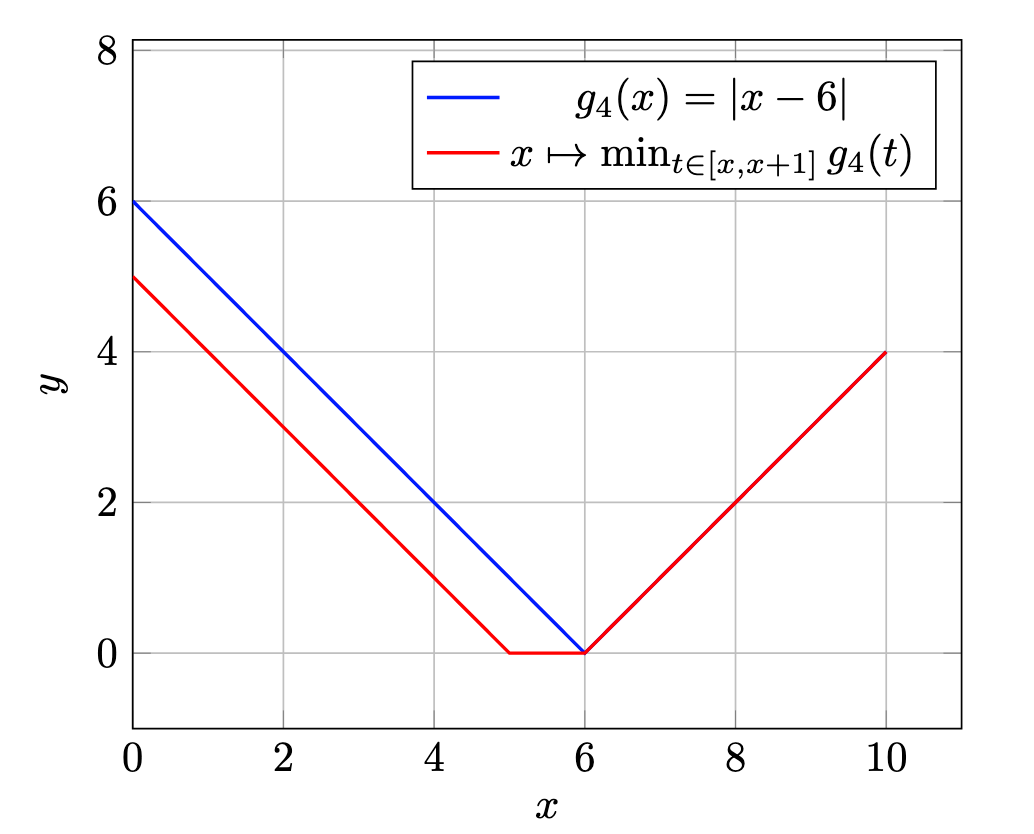
\includegraphics[width=\linewidth]{slides/g_4.png}
		\end{minipage}\hfill
		\begin{minipage}{0.24\textwidth}
			\centering
			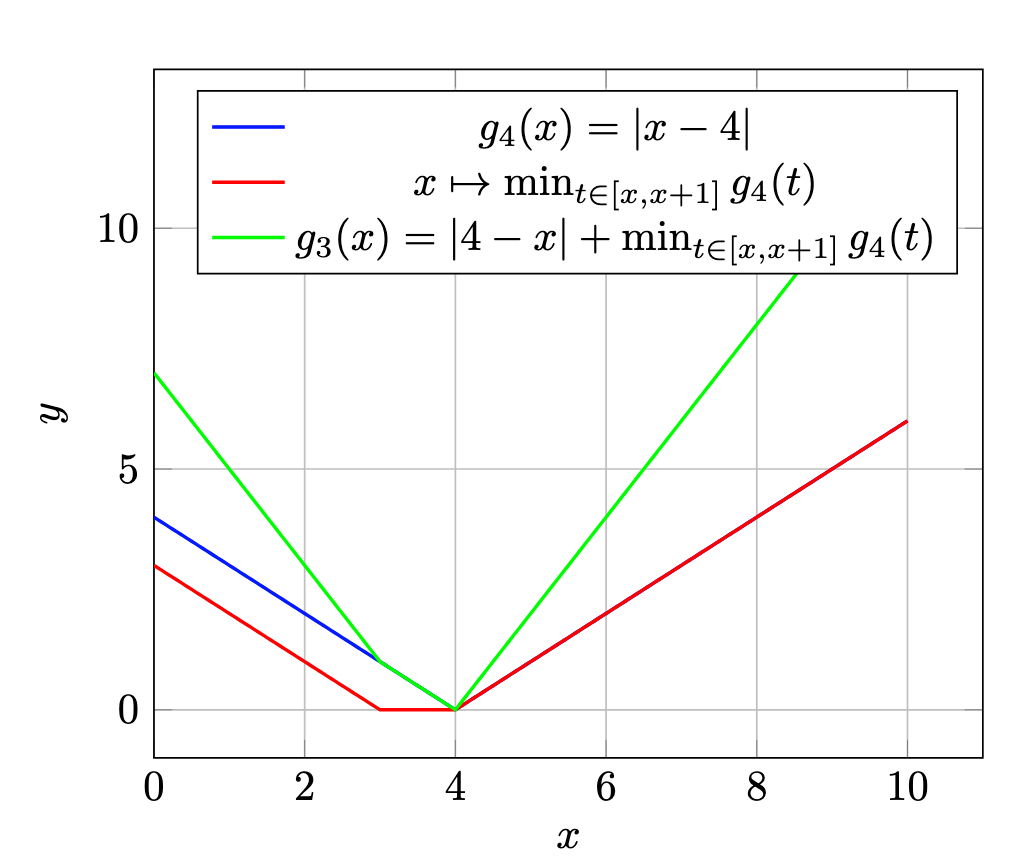
\includegraphics[width=\linewidth]{slides/g_3.png}
		\end{minipage}
		\caption{Illustration of a run of the algorithm on Example \ref{stampcomp}.}
		\label{fig:g_4}
	\end{figure}
	
	We construct $g_2$ similarly, by summing the contribution of the next timestamp aligning cost, $|x - 2|$, to  $\min_{x' - x \in [2,4]}g_3(x')$. 
	We now find an orange segment in the second component. This is used to demarcate any additional segments in  $\min_{x' - x \in [a_i, b_i]}g_{i-1}(x')$ not present in $g_{i-1}$. 
	We see the effect of the $\min$ operation is to attach a segment with the same length as the $i$th static interval constraint, at the lowest point of $g_{i-1}$. 
	We continue similarly : The next black graph is a translation of the previous blue one, with an orange line segment or the same length as the next static interval constraint inserted at the lowest point, and the next green graph is $|x-\sigma_i|$ in the new domain, and summing these two gives the next blue graph. 
	As these are all piecewise linear graphs, summing is simply incrementing the slopes of all the segments of the black-orange curve by one if they're to the right of $\sigma_i$, and by minus one if they're to the left, and translating the height up as needed. 
	%Clearly the orange, black and green segments of the next graph are obtained like this, and $g_4$ is their sum. 
	
	The procedure for constructing $g_4$ is identical, and now finally we see that the minimum cost of $2$ is achieved in $g_4$ by paying at time 6. 
	Now, we know the contribution of the $(pay,6)$ to the error is 0, so this means we can deduce the corresponding value in $g_3$ must have been 2, achieved when $dec$ fires at 5. 
	We can backtrack in this manner to build an optimal alignment, such as in this case, $(reg,1)(check,3)(dec,5)(pay,6)$. 
\end{example}

With this context, we present the following algorithm that progressively calculates the graphs of $g_i$ (which are a continuous, piecewise linear, convex function admitting $+\infty$ as limit at $\pm\infty$, represented as lists of segments, each characterised by their slopes and x-projections of endpoints) each round, and claim it is both correct and efficient. 
The algorithm precisely executes the above procedure, where the subfunction \textsc{graphMin} takes $g_i(d)$ and outputs $$\min_{d-d' \in [a,b]} g(d') = \begin{cases}
	g(d-a) & l + a \leq d < m + a \\
	g(m) & m+a \leq d \leq m' + b \\
	g(d+b) & m' + b < d \leq h + b   \\
\end{cases}$$ Which is exactly the process of taking the last blue graph and creating the next orange-black graph, and subfunction \textsc{graphAddMod} takes $\min_{d-d' \in [a,b]} g(d')$ and adds $|d - \sigma_{i+1}|$ to it, i.e., adding the green component. The proof of the nature of the functions and how they are constructed will be given in the next section \ref{tree_like structures} when we discuss more general cases. Lastly, the \textsc{backTrack} algorithm backtracks through the list of graphs $\{g_i\}_n$ constructed to reverse engineer a word that aligns with the minimal cost calculated. Again, a more detailed algorithm for backtracking will be proposed in the next section \ref{tree_like structures}. 

\begin{figure}
	\removelatexerror
	\begin{algorithm}[H]
		\caption{$d_t$ Algorithm}
		\label{StampAlgo}
		\SetAlgoLined
		\LinesNumbered
		\KwIn{$\sigma$, $SI$}  
		\KwOut{$cost = \min_{x \in \mathcal{L}(N)}{d_t(x, \sigma)}$, $\gamma \in \mathcal{L}(N)$ such that $d_t(\gamma, \sigma) = cost$}
		\KwData{$graph = \{(left, slope, right) | graph[i].left = graph[i-1].right\}$}
		\SetKwProg{Fn}{Procedure}{:}{end}

		\Fn{StampOnlyAlgo($\sigma, SI$)}{
			Initialise System \\
			$[a, b] \gets SI[i]$ \\
			$graph \gets \{(a, 0, b)\}$ \\
			\textsc{graphAddMod}($graph, \sigma[0]$) \\
			$graphlist \gets \{graph\}$ \\ 
			$i \gets 1$ \\
			$cost \gets |a - \sigma[0]|$ \\ 
			\While{$i < |sigma|$}{
				$[a, b] \gets SI[i]$ \\ 
				\textsc{graphMin}($graph, a, b$) \\ 
				\textsc{graphAddMod}($graph, \sigma[i]$) \\
				$graphlist.append(graph)$ \\
				$cost \gets cost + |a - \sigma[i]|$ \\
			}
			$i \gets 0$ \\
			$s \gets graph[0].slope$ \\
			
			\While{$graph[i].slope < 0$}{
				$s \gets graph[i].slope$ \\
				$cost \gets cost + s * (graph[i].right - graph[i].left)$ \\
				$i \gets i + 1$ \\
			}
			$\gamma \gets \textsc{backTrack}(\sigma, graphlist, cost, SI)$ \\
			\Return{$cost, \gamma$}
		}
	\end{algorithm}
\end{figure}

\begin{theorem}\label{StampAlgoCorr}
	Algorithm \ref{StampAlgo} is correct, i.e., it outputs a valid execution
	$\gamma \in \mathcal{L}(N)$ which minimizes the distance $d_t(\gamma, \sigma)$
	to the trace $\sigma$.
\end{theorem}
		
\begin{remark} Note that the subfunctions \textsc{graphMin} and  \textsc{graphAddMod} both run through the list of segments of the graph once each, and hence are linear in the sizes of their inputs, and Algorithm \ref{StampAlgo} calls each of these subfunctions once for each letter of the observed trace, each time on a graph with size linear in the current prefix.  
	So the cost calculation section of Algorithm \ref{StampAlgo} has quadratic time complexity in the size of the input. 
	
	The subfunction \textsc{backTrack} runs a binary search on each stored graph in $graphlist$ to find a trace in the language that does indeed give the minimum cost, letter by letter, and so overall takes $O(n \log(n))$ time, keeping the overall time complexity  $O(n^2)$ where $n = |\sigma|$.
\end{remark}


\subsection{Generalisation for Tree-like Models} \label{tree_like structures}

As discussed previously, we have developped an algorithm to solve the alignment problem for sequential models by building a recurrent link between two consecutive levels. It appears that this approach is really general and can be adapted to more complex models like tree-like structures. Let us first define what we mean by tree-like models.

% We are given a process model $N$, an observed trace $\sigma$, and its underlying sequential causal process $CN = (B, E, G)$ with homomorphism $p$ for the untimed run of $\sigma$ on $N$. 
% We express the cost of aligning a prefix of $\sigma$ to some timing function $\tau$ on the truncation of the sequential causal process up to the $i$th transition, call it $cost$. 
% $$cost(\tau|_i) = \sum_{j = 1}^{i} |\tau_j - \sigma_j| = |\tau_i - \sigma_i| + cost(\tau|_{i-1})$$
% Observe that the minimum cost to align $\sigma$ depends on exactly two things, the cost of aligning the last stamp, and the minimum cost of aligning the $n-1$ length prefix of $\sigma$, such that the last and second last timestamps obey the last static interval constraint.  
% This suggests that the minimal cost of aligning prefixes of $\sigma$ to prefixes of the model can be recursively calculated as a function of the last timestamp in the alignment of a given prefix. 

% Let $g_i(d) = \min\{cost(\tau|_i) \textit{ with } \tau|_i \in \mathcal{L}^i(N) \wedge \tau_i = d\} $. 

% Now, the recursive relation $g$ functions obey is : 
% $$g_{i+1}(d) = |d - \sigma_{i+1}| + \min_{d-d' \in [a,b]} g_i(d')$$
% If we can calculate the family of functions $\forall i \leq n : g_i$ efficiently, then the minimal cost for aligning $\sigma$ to $N$ is simply $\min_{d} g_n(d)$. 

% This relation holds on the fact that the minimal aligning cost of a big sequence can be calculated from the minimal aligning cost of its subsequence : By setting $d$, the subsequence needs to be aligned with its last execution moment set to $d' \in [d-b,d-a]$, which is exactly a subproblem.
% Since this property is preserved even in tree-like structures, we expect to find similar result for this kind of model.
\begin{definition}[Tree-like Time Petri Net]
    Let N = (P,T,F,SI,$\Sigma,\lambda,M_0,M_f$) be a Time Petri Net. N is Tree-like if it's connected, acyclic and \[\forall t \in T, |t^{\bullet}| \geq 1 \textit{ and } |{}^{\bullet}t| = 1,\] \[\forall p \in P, |p^{\bullet}| \leq 1 \textit{ and } |{}^{\bullet}p| \leq 1.\]
    N is so called Tree-like Time Petri Net.
\end{definition}
Tree-like models are a natural generalisation of sequential models, where activities can branch out into multiple parallel threads of execution and are executed separately since.
The fundamental difference of tree-like models comparing to sequential models is its dependencies between 
higher and lower layers. Precisely, the firing time of an event in a lower layer may affect the firing time of multiple events in the higher layer and by consequence, to fix the firing time of an transition in the lower layer, we may need to take care of multiple events in the higher layer.

\begin{example}\label{Tree-like Time Petri Net}
		We show here an example of Tree-like Time Petri Net and one of the 
		possible traces respecting the process' action order $\sigma = (a,3)(b,10)(c,4)(d,12)(e,15)$.
		\vspace{0.4cm}

		\adjustbox{scale = 0.8}{
			\begin{tikzcd}
				{} & {} & {} & {} & \Huge\bigcirc & {\fbox{d}} & \Huge\bigcirc \\
				{} & {} & \Huge\bigcirc & {\fbox{b}} & {} & {} &	\\
				\Huge\bigcirc & {\fbox{a}} & {} & {} & \Huge\bigcirc & {\fbox{e}} & \Huge\bigcirc \\
				{} & {} & \Huge\bigcirc & {\fbox{c}} & \Huge\bigcirc & {} &	\\				
				{} & {} & {} & {} & {} & {} & \\
				\arrow[from=3-1, to=3-2]
				\arrow[from=3-2, to=2-3]
				\arrow[from=3-2, to=4-3]
				\arrow[from=2-3, to=2-4]
				\arrow[from=4-3, to=4-4]
				\arrow[from=4-4, to=4-5]
				\arrow[from=2-4, to=1-5]
				\arrow[from=2-4, to=3-5]
				\arrow[from=3-5, to=3-6]
				\arrow[from=1-5, to=1-6]
				\arrow[from=1-6, to=1-7]
				\arrow[from=3-6, to=3-7]
				\arrow["{[1,4]}"{description, pos= 0.8}, draw=white, from=4-2, to=3-2]
				\arrow["{[2,3]}"{description, pos= 0.8}, draw=white, from=3-4, to=2-4]
				\arrow["{[5,7]}"{description, pos= 0.8}, draw=white, from=5-4, to=4-4]
				\arrow["{[1,1]}"{description, pos= 0.8}, draw=white, from=2-6, to=1-6]
				\arrow["{[5,6]}"{description, pos= 0.8}, draw=white, from=4-6, to=3-6]
			\end{tikzcd}
		}
	Now, the question is how to align $\sigma$ to the model with minimum cost. 

	We can firstly try to align $\sigma$ to the model by greedy approach : From left to right, 
	at each transition, we try to fix its firing time with minimum cost while respecting the static interval constraint. We start by aligning the root of the tree,
	which is transition $a$. Since $a$ is executed at 3, which is between 1 and 4, we don't need to 
	change its execution moment. 
	\[\sigma_{aligned} = (a,3)...\]

Then, we move to $a$'s children :
$b$ must be fired between 2 and 3 after $a$, so the minimal cost of correcting $b$'s execution moment is 4,
by setting it to 6. Similarly, $c$ must be fired between 5 and 7 after $a$, so we set its execution moment to 8, 
which costs us 4. 
\[\sigma_{aligned} = (a,3)(b,6)(c,8)...\]
Following the same reasoning, $d$ must be fired at 7 and $e$ at 12, which costs us 5 and 3 respectively.
\[\sigma_{aligned} = (a,3)(b,6)(c,8)(d,7)(e,12)\]
Finally, the total cost of aligning $\sigma$ with the Petri net is 16. Now, by trying to get something 
better from $\sigma_{aligned}$, we found a better alignment with cost of 15 which is
\[\sigma_{aligned}' = (a,4)(b,7)(c,9)(d,8)(e,13)\]
by remarking that shifting the execution moment of $a$ from 3 to 4 reduces the total cost by 3 (on nodes $b, c$ and $d$) while increasing the cost by 2 (on $a$ and $e$).
\end{example}

This example proved that the local optimal choice on a higher layer may not lead to the global optimal solution, we need to consider the effect of changing a node's execution moment on all its descendants.
Hence, the advantage of the recurrent relation used in sequential models which computes the alignement cost with respect to the effects on the nodes behind. 

\subsection*{Notations and Results}
We are given a model $N$ represented as a Tree-like Time Petri Net, an observed trace $\sigma$, and its underlying sequential causal process $CN = (B, E, G)$ with homomorphism $p$ for the untimed run of $\sigma$ on $N$. 
As there are no choices for either firing one transition or another in the model, the causal process associated to $\sigma$ exactly matches the model.

In the following, we focus on the execution moment of every transition and the places don't play any important role here, we will refer to every transition $i$ as \textit{node} and $i^{\bullet\bullet}$ or $\text{Child}(i)$ as set of its \textit{children}.
Considering the causal process associated to the observed trace $\sigma$ which is tree-like, we denote by $\sigma_i$ the execution moment of node $i$ in $\sigma$ and by $[a_i, b_i]$ its static interval constraint.
\begin{proposition}
	Let $i$ be a node in the tree-like causal process, and let $g_i(x)$ be the minimum cost of aligning the sub-process rooted at ${}^\bullet i$ when $i$ is fired at time $x$. Then, $g_i(x)$ obeys the following recurrent relation :
    \begin{align*}
        \begin{split}
            g_{i}(x) & = |\sigma_{i}-x| + \min\Biggl\{\sum_{\substack{j \in \text{Child}(i) \\ x_{j}-x\in[a_{j},b_{j}]}}g_{j}(x_{j})\Biggr\} \\
            & = |\sigma_{i}-x| + \min\Biggl\{\sum_{\substack{j \in \text{Child}(i) \\ x_{j}\in[x+a_{j},x+b_{j}]}}g_{j}(x_{j})\Biggr\}
        \end{split}
    \end{align*}
\end{proposition}
So, in order to have the minimal alignment cost at node $i$, the $(x_j)_{j \in \text{Child}(i)}$ must be chosen such that the sum of the alignment costs of all its children is minimized, while respecting their static interval constraints. But there are no constraintes between the choices of $x_j$, so we can minimize each $g_j(x_j)$ independently. Therefore, we have the following relation :
\begin{proposition}
    \begin{align*}
        \begin{split}
            g_{i}(x) & = |\sigma_{i}-x| + \min\Biggl\{\sum_{\substack{j \in \text{Child}(i) \\ x_{j}\in[x+a_{j},x+b_{j}]}}g_{j}(x_{j})\Biggr\} \\
            & = |\sigma_{i}-x| + \sum_{j \in \text{Child}(i)}\min_{x_{j}\in[x+a_{j},x+b_{j}]}\{g_{j}(x_{j})\}\\
        \end{split}
    \end{align*}
\end{proposition}

Now, suppose that we get access 
to each value of $g_{root}(x)$ as $x$ varies. Then, the minimal cost of aligning the 
whole sequence with the Petri net is $\min_{x\in[a_i,b_i]}\{g_{i}(x)\}$, which 
is exactly the least cost to set the root's execution moment to a value between
$a_{root}$ and $b_{root}$ and to align all of its sub-trees.

\begin{proposition}
    The minimal cost of aligning the sequence with the whole Petri net 
    is \[\min_{x\in[a_{root},b_{root}]}\{g_{root}(x)\}\]. 
\end{proposition}

We are now interested in the nature of the function $g_{i}(\cdot)$ to be able to compute it effectively. 
The two following results give us some key properties of these functions.

\begin{lemma}\label{tree-like}
    For any node $i$ of the tree, the function $g_{i}(\cdot)$ is a continuous, convex, 
    piecewise linear, and diverges to $+\infty$ at $\pm\infty$.
\end{lemma}
\begin{proof}
	We show by induction the property : For every node $u$ of the 
	tree, $H_i: g_{i}(\cdot)$ is a continuous, convex, piecewise linear function 
	which tends to $+\infty$ at $\pm\infty$.
	Initially, if $i$ is a leaf, $H_i$ is true directly since 
	$g_{leaf}(x) = |\sigma_{leaf} - x|$ is an absolute value function. 
	We climb up the tree and suppose that for every 
	$j \in \text{Child}(i)$, $H_j$ is true. The two first points above show that
	\begin{equation}
			\begin{split}
					g_{i}(x) & = |\sigma_{i}-x| + \sum_{j \in \text{Child}(i)}\min_{x_{j}\in[x+a_{j},x+b_{j}]}g_{j}(x_{j}) \\
					& = |\sigma_{i}-x| + \sum_{j \in \text{Child}(i)}h_j(x)
			\end{split}
	\end{equation}
	where $h_j : x\mapsto \min_{x_{j}\in[x+a_{j},x+b_{j}]}g_{j}(x_{j})$. 
	By induction hypothesis, $g_{j}(\cdot)$ is a continuous, convex, piecewise linear function 
	which tends to $+\infty$ at $+\infty$ and $-\infty$. According to 
	Lemma~\ref{lem:important} shown further below, $h_j$ also possesses these same properties. 
	Finally, since the sum of continuous, convex, piecewise linear functions 
	which tend to $+\infty$ at $+\infty$ and $-\infty$ is also a 
	function of the same type, 
	we deduce that $g_{i}(\cdot)$ also possesses these properties. Hence, the result.
\end{proof}

\begin{corollary} 
    Let $g$ a continuous, convex, piecewise linear function whose limits 
    at $+\infty$ and $-\infty$ exist and are $+\infty$. There exist then $x_{0}$ and 
    $x_{1}$ such that $g$ decreases in $]-\infty,x_{0}]$, constant in $[x_{0},x_{1}]$ 
    and increases in $[x_{1},+\infty[$. We refer to these as decreasing, stationary and 
    increasing zones. As a consequence, every function $g_{i}(\cdot)$ possesses these 
    proprieties.
\end{corollary}

With these properties in mind, let's pick up the example \ref{Tree-like Time Petri Net} again to illustrate how to compute these functions in practice. 
\begin{example}
	We consider again the Tree-like Time Petri Net from example \ref{Tree-like Time Petri Net} and the observed trace $\sigma = (a,3)(b,10)(c,4)(d,12)(e,15)$.
	We start by computing the functions $g_{d}(x)$, $g_{e}(x)$ and $g_{c}(x)$ associated to the leaves $d,e$ and $c$.
	Since they don't have any children, we have :
	\[g_{d}(x) = |\sigma_{d}-x| = |12-x|\]
	\[g_{e}(x) = |\sigma_{e}-x| = |15-x|\]
	\[g_{c}(x) = |\sigma_{c}-x| = |4-x|\]
	Both functions are piecewise linear with a vertex at $\sigma_{d},\sigma_{e}$ and $\sigma_{c}$ respectively. 
	Then, we move up to node $b$ to compute $g_{b}(x)$.
	Using the recurrent relation, we have :
	\[g_{b}(x) = |\sigma_{b}-x| + \min_{x_{d}\in[x+1,x+1]}\{g_{d}(x_{d})\} + \min_{x_{e}\in[x+5,x+6]}\{g_{d}(x_{e})\}\]
\end{example}
To compute $g_{b}(x)$, we first need to compute the two minimizations. The following lemma will show us how to compute them from the knowledge of $g_{d}(\cdot)$ and $g_{e}(\cdot)$.
\begin{lemma} \label{lem:important} 
    For all real couple a,b s.t a $\leqslant$ b, and for all continuous, convex, 
    piecewise linear function f which tends to $+\infty$ at $+\infty$ and 
    $-\infty$, \[ g : x\mapsto \min_{t\in[x+a, x+b]}f(t) \] is also a continuous, 
    convex, piecewise linear function having $+\infty$ as limit at $\pm\infty$.
\end{lemma}
\begin{proof}
    We present here a method for obtaining the graph of $g$ from the graph of $f$. A rigorous proof can then be easily deduced. 

    Now, since $f$ is continuous, convex, piecewise linear, Corollary 1 implies the existence of two real numbers $x_0$ and $x_1$ such that $f$ decreases in $]-\infty,x_0]$, constant in $[x_0,x_1]$, increasing in $[x_1,+\infty[$. Then, the minimum of $f$ in the interval $[x+a, x+b]$ that slides from left to right as $x$ increases can be estimated based on the relative position between $[x_0,x_1]$ and $[x+a, x+b]$. We distinguish three cases: 
    \begin{itemize}
        \item[$\blacksquare$] When the intersection $[x_0, x_1] \cap [x + a, x + b]$ is nonempty, we have
\[
g(x) = \min_{t \in [x + a, x + b]} f(t) = \min_{\mathbb{R}} f,
\]
    since the interval $[x + a, x + b]$ contains points where $f$ attains its global minimum. Therefore, the graph of $g$ over the interval $[x_0 - b, x_1 - a]$ is a horizontal segment at height $y = \min_{\mathbb{R}} f$. That is, the graph can be obtained by shifting the graph of $f$ restricted to $[x_0, x_1]$ left by $b$ units and extending it to the right by $(b - a)$ units.
    
    \item[$\blacksquare$] When $x + b \leq x_0$, the interval $[x + a, x + b]$ lies entirely to the left of $x_0$, and $f$ decreases in this interval. Hence,
    \[
g(x) = \min_{t \in [x + a, x + b]} f(t) = f(x + b).
\]
    The graph of $g$ in the interval $]-\infty, x_0 - b]$ is obtained by shifting the graph of $f$ restricted to $]-\infty, x_0]$ left by $b$ units.
        
    \item[$\blacksquare$] When $x_1 \leq x + a$, the interval $[x + a, x + b]$ lies entirely to the right of $x_1$, and $f$ increases in this interval. Hence,
\[
g(x) = \min_{t \in [x + a, x + b]} f(t) = f(x + a).
\]
    The graph of $g$ in the interval $[x_1 - a, +\infty[$ is obtained by shifting the graph of $f$ restricted to $[x_1, +\infty[$ left by $a$ units.
    \end{itemize}
    Finally, $g$ can be drawn correctly as shown in an example illustrated in Figure \ref{fig:Graph_g} below.
    \begin{figure}[H]
        \centering
        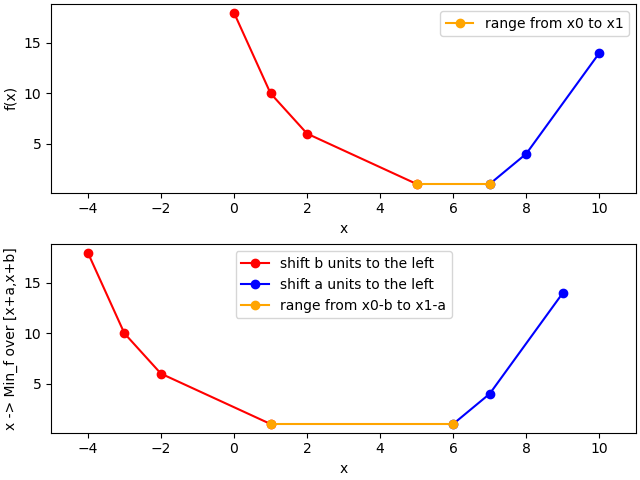
\includegraphics[width=1\linewidth]{images/translation.png}
        \caption{Example with $x_0$ = 5, $x_1$ = 7, a = 1, b = 4}
        \label{fig:Graph_g}
    \end{figure}
    Graphically, it is clear that $g$ is also a continuous, convex, piecewise linear function that has $+\infty$ as limit at $\pm\infty$. A rigorous proof can be driven by formalizing these arguments mentioned above and justifying the convexity of $g$ very easily.
\end{proof}
With all these elements, we can now compute $g_{b}(x)$ and then $g_{a}(x)$ without any difficulty. To finish the example \ref{Tree-like Time Petri Net}, we have :
\begin{equation}
	\label{eq:5}
	g_{a}(x) = |3 - x| + \min_{x_b\in[2+x,3+x]}g_{b}(x_b) + \min_{x_c\in[5+x,7+x]}g_{c}(x_c)
\end{equation}

\begin{figure}[H]
    \centering
    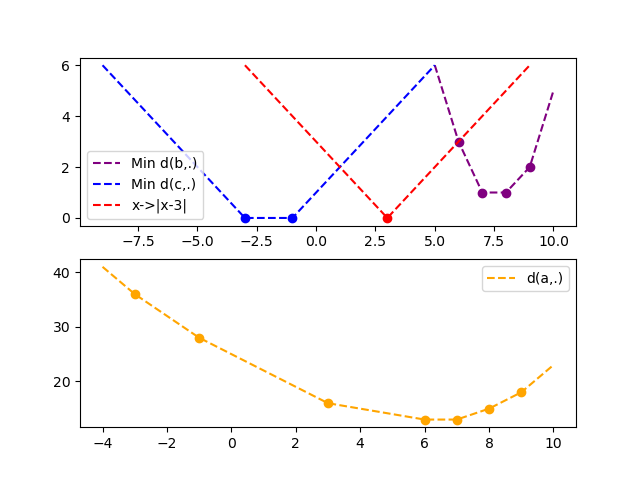
\includegraphics[width=1\linewidth]{images/d_a.png}
    \caption{Noting $\forall \tau \in T, g_{\tau}(\cdot) = d(\tau,\cdot)$, cost function $x\mapsto g_{a}(x)$}
    \label{fig:d(a,.)}
\end{figure}

Finally, we obtain the cost function for the root \ref{fig:d(a,.)}. Zooming in a bit, we see that the graph attains its global minima on the interval $[6,7]$ but it is not the result directly. 
The first transition is fired between 1 and 4, the minimal cost of our alignment problem is \[\min_{x\in [1,4]}g_{a}(x)\] which is 15, attains at $x = 4$. 
Looking back to the equation \eqref{eq:5}, we can deduce that the best alignment is obtained by setting $a$ to 4, then $b$ will be set to $x_{b}$ which minimizes $g_{b}(\cdot)$ over $[2+x,3+x]$. 
Since $x = 4$, $[2+x,3+x] = [6,7]$ and the minimum of $g_{b}(\cdot)$ over this interval is attained at 7. 
So $x_{b}$ is 7. Similarly, $x_{c}$ will be set to 9, $x_{d}$ to 8 and $x_{e}$ to 13. We then get the aligned trace 
\[\sigma_{aligned}' = (a,4)(b,7)(c,9)(d,8)(e,13)\]
with a total cost of 15. This is exactly the result we found above. 

To sum up the method shown above, the pseudocode \ref{alg:Cost_function_computing} of the algorithm is to compute the cost functions $g_{i}(\cdot)$ for all nodes $i$ in a bottom-up fashion and to find the aligned trace with minimum cost. The following theorem states the correctness of the algorithm.
\begin{theorem}
		The algorithm \ref{alg:Cost_function_computing} computes the optimal alignment of a timed trace $\sigma$ to a tree-like Time Petri Net $N$ under Stamp Only Distance and the corresponding minimal cost.
\end{theorem}

\begin{proof}
	Before proving the correctness of the algorithm, since the net is tree-like, so confusion-free, there is no need to worry about the condition of urgency. Therefore,
	three conditions cited in the theorem \ref{thm35} are reduced to one : The execution moment of each transition must respect its static interval constraint.	Now, we prove the correctness of each function used in the algorithm.
	\begin{itemize}
		\item Firstly, we prove the correctness of the function $Compute\_cost\_function$ by induction on the height of the tree.
		Initially, if $i$ is a leaf, the function returns $g_{i}(x) = |\sigma_{i} - x|$ which is correct (Line 4).
		By defining the height of a node its biggest distance to a leaf in its subtree, the inital case was showing the that the function works for nodes of height 0.
		We climb up the tree and suppose that for every node $j$ of height less than $h$, the function returns the correct cost function $g_{j}(\cdot)$.
		Let $i$ be a node of height $h$. All children of $i$ have height at most $h-1$, so by induction hypothesis, the function returns the correct cost functions $g_{j}(\cdot)$ for all $j \in \text{Child}(i)$.
		Then, according to the recurrent relation shown above, the function computes correctly $g_{i}(\cdot)$ from these functions (Lines 7-13). So the function works for nodes of height $h$. Hence, its correctness for all nodes of the tree.
		\item Now we prove the correctness of the function $Align\_trace$ once every cost function $g_{i}(\cdot)$ is computed.
		According to the recurrent relation shown above \[g_{i}(x) = |\sigma_{i}-x| + \sum_{j \in \text{Child}(i)}\min_{x_{j}\in[x+a_{j},x+b_{j}]}\{g_{j}(x_{j})\}\]
		the execution moment of each node $j$ in the optimal alignment can be computed from the execution moment of its parent (to minimize the cost).
		By following the structure of Depth-First Search (Lines 16-22), we suppose that the parent of the $root$ is executed at 0, then we can compute the execution moment of each node in the optimal alignment correctly. Hence, the correctness of the function $Align\_trace$.
		\item The correctness of $Main$ is then straightforward since it just calls the two previous functions in order (Lines 24-27).
	\end{itemize}
\end{proof}

To provide some complexity analysis and conclude this section, we note that each function $g_i(\cdot)$ is a continuous, convex, piecewise linear function
which can be characterized by its leftmost and rightmost slopes and a set of points located at positions where the slopes change. Also, by summing these functions, the sum is a function of the same type and its slopes change only at points where the slope of one of its components changes. 
Thus, it is possible to calculate an upper bound for the number of breakpoints of the functions $g_{u}(\cdot)$ for all node $u$.

\begin{lemma}\label{Encadrement}
For a node $u$, let $S_{g_{u}(\cdot)}$ denote the set of breakpoints (points where slope changes) of the function $x \mapsto g_{u}(x)$, and $S_{\min g_{u}(\cdot)}$ for $x \mapsto \min_{x_u \in [a_u+x, b_u+x]} g_{u}(x_u)$. Then:
\begin{enumerate}
    \item $|S_{\min g_{u}(\cdot)}| \leq |S_{g_{u}(\cdot)}|+1 $
    \item $|S_{g_{u}(\cdot)}| = |\{\sigma_u\}\cup \bigcup_{j\in\text{Child}(u)}S_{\min g_{j}(\cdot)}|$
    \item $|S_{\min g_{u}(\cdot)}| \leq 2|T_u|$ where $T_u$ is the set of transitions of the subtree whose root is ${}^\bullet u$.
\end{enumerate}
\end{lemma}

\begin{proof}
    Scholium:
    \begin{enumerate}
        \item Based on the proof of \autoref{lem:important}, the graph of 
        $x\mapsto\min_{x_u \in [a_u+x,b_u+x]}g_{u}(x_u)$ can be obtained by 
        translating the graph of $x\mapsto g_{u}(x)$ and extending its stationary 
        zone. As a result, this extension of the stationary zone can at most add 
        one more point to $S_{\min g_{u}(\cdot)}$ compared to $S_{g_{u}(\cdot)}$.
        \item We know that 
        \[g_{u}(x) = |x-\sigma_u| + \sum_{j\in \text{Child}(u)}\min_{x_j \in [a_j+x,b_j+x]}g_{j}(x_j)\] 
        and by adding the affine functions, the slopes add up. Therefore, the sum, 
        which is also a piecewise linear function, can change its slopes only at 
        points where the slope of one of its components changes. Hence the result.
        \item We show by induction the property : For every node $u$ of the 
        tree, \[H_u: |S_{\min g_{u}(\cdot)}| \leq 2|T_u|.\] 
        Initially, if $u$ is a leaf, $H_u$ is true directly. 
        We climb up the tree and suppose that for every 
        $j \in \text{Child}(i)$, $H_j$ is true. The two first points above show that
        \begin{equation}
            \begin{split}
                |S_{\min g_{u}(\cdot)}| \leq 1 + |S_{g_{u}(\cdot)}| 
                & = 1 + |\{\sigma_u\}\cup \bigcup_{j\in\text{Child}(u)}S_{\min g_{u}(\cdot)}| \\
                & \leq 1 + |\{\sigma_u\}| + \sum_{j\in\text{Child}} |S_{\min g_{u}(\cdot)}| \\
                & \leq 2 + \sum_{j\in\text{Child}(u)}2|T_j|\\
                & = 2|T_u|
            \end{split}
        \end{equation}
        By deduction, the result is true for all nodes of the tree. Hence, the result. 
    \end{enumerate}
\end{proof}

We can now conclude by giving the pseudocode of the algorithm for tree-like models and its complexity \ref{alg:Cost_function_computing}. 
\begin{figure}[t]
	\removelatexerror
	\begin{algorithm}[H]
		\label{alg:Cost_function_computing}
		\caption{Aligning a timed trace with a Tree-like Time Petri Net under Stamp Only Distance}
		\SetAlgoLined
		\LinesNumbered
		\KwIn{A tree-like Time Petri Net N = (P,T,F,SI,$\Sigma,\lambda,M_0,M_f$) modelized by $G = (V,E)$ where 
		$V = T$ and $(t_i,t_j)\in E$ iff $t_j \in t_i^{\bullet\bullet}$ and a timed trace $\boldsymbol{\sigma} = (a_1,t_1)(a_2,t_2)...(a_n,t_n)$}
		\KwOut{The minimal cost of aligning $\boldsymbol{\sigma}$ with N and the aligned trace $\boldsymbol{\sigma_{aligned}}$}
		\KwData{$\sigma_{aligned} \gets [], x_{parent} \gets 0$}
		\SetKwProg{Fn}{Function}{:}{end}
			\Fn{Compute\_cost\_function($node$)}{
					\lIf{$g_{node}$ is calculated}{
							\Return{$g_{node}(x)$}
					}
					\ElseIf{$node$ is a leaf}{
							\Return{$g_{node}(x) \gets |\sigma_{node} - x|$}\\
					}
					\Else{
							$g_{node}(x) = |\sigma_{node} - x|$\\
							\ForEach{$child$ in Child($node$)}{
									$g_{child}(x)$ $\gets$ Compute\_cost\_function($child$)\\
									$min\_g_{child}(x)\gets \min_{x_{child} \in [a_{child}+x,b_{child}+x]}g_{child}(x_{child})$\\
									$g_{node}(x) \gets g_{node}(x) + min\_g_{child}(x)$
							}
							\Return{$g_{node}(x)$}
					}
			}

			\Fn{Align\_trace($node$, $x_{parent}$)}{
					$x_{node} \gets argmin_{x_{node}-x_{parent} \in [a_{node},b_{node}]}g_{node}(x_{node})$\\
					\If{$node$ is a leaf}{
							\Return
					}
					\ForEach{$child$ in Child($node$)}{
							Align\_trace($child$, $x_{node}$)
					} 
			}

			\Fn{Main()}{
					$root \gets$ root of the tree\\
					$g_{root}(x) \gets$ Compute\_cost\_function($root$)\\
					$cost \gets \min_{x \in [a_{root},b_{root}]}g_{root}(x)$\\
					Align\_trace($root$, 0)\\
					\Return{$cost$, $\boldsymbol{\sigma_{aligned}}$}
			}
	\end{algorithm}
\end{figure}

The complexity of the algorithm mainly depends on the 
calculation of $g_{node}(x)$ for each node of the tree. For 
a node $u$, calculating $g_{u}(x)$ requires summing the 
contributions of its children, which can be done in 
$O(|\text{Child}(u)| \cdot |S_{g_{j}(\cdot)}|)$ time, where 
$j \in \text{Child}(u)$. Since $|S_{g_{j}(\cdot)}|$ is bounded 
by $2|T_j|$ according to the previous lemma, the time 
complexity for computing $g_{u}(x)$ becomes 
$O(|\text{Child}(u)| \cdot |T_j|)$. Summing this over 
all nodes in the tree, we find that the overall time 
complexity of the algorithm is $O(|T|^2)$, where $|T|$ 
is the number of transitions in the Petri net. This quadratic 
complexity arises from the need to compute and store the cost 
functions for each node and their children.

Function Align\_trace traverses the tree once, and at each node,
determines the optimal execution moment based on the precomputed cost functions 
in $O(1)$ time. In total, this function runs in $O(|T|)$ time and 
so the overall time complexity of the algorithm is
$O(|T|^2) + O(|T|) = O(|T|)^2$. 


\section{Results and Algorithm : Delay Edits}\label{4}
Delay edits provide a new way of thinking about transformations over time-series, and inspire a new way of viewing timing functions over causal processes. 
There is of course the standard definition, $\tau : E \to \mathbb{R}^+$ that assigns to each event a timestamp that records exactly when the event occurs. 

Instead, thinking along the lines of durations between events occurring, we will often benefit from considering the following representation when speaking about delay moves, defined as to view a timed word not in terms of its absolute timestamps, but by the delays between them. 

\begin{definition}[Flow Function]
	Given a causal process $(CN, p)$ over $N$, where $CN = (B, E, G)$, and a (not necessarily valid) timing function $\tau : E \to \mathbb{R}^+$, we first define the \textit{flow} function of $\tau$, $f_{\tau} : E \to \mathbb{R}^+$ such that 
	$$f_{\tau}(e) = \begin{cases} 
		\tau(e) & \pre \pre e = \emptyset\\
		\tau(e) - \tau(e') &e' \in   \pre \pre e,\\ & \tau(e') = \max\limits_{e'' \in \pre \pre e} {\{\tau(e'')\} \cup \{0\}}\\
	\end{cases}
	$$
	
\end{definition}

\begin{example}\label{wordandflow}
	Consider again the model in example \ref{TPN}.
	Say we want to align  $w = (reg, 1)(et, 2)(ct, 5)(dec, 6)(rej, 8)$ to $N$.  
	Consider the values the clock takes during a faulty ``execution'' $reg \to 1, et \to 1, ct \to 4, dec \to 1, rej \to 2$. This is the flow function. 
\end{example}

Note that $e'$ as defined here is the latest causal predecessor of $e$
%, i.e., it is the firing of $e'$ that enabled $e$
. 
Hence, $f_\tau$ as defined produces exactly the time durations that the guards of each transition in the model checks, i.e. the clock function values during the run. 

As defined, we see that if a word is in the language of the model, then its $f$ function maps events to values that lie within the event's static interval constraint.
This condition is unfortunately not sufficient due to urgency which determines the only firable transition, but it is quite close to the exact condition necessary for a word to be in the language of a time Petri net. 

Also note that given the underlying causal process and the resulting $f_\tau$, we can reconstruct $\tau$ quite straightforwardly as $\forall e \in E : \tau(e) = \sum_{e' \leq_G e} f_\tau(e')$.

\begin{lemma}[Delay only distance : $d_\theta$]\label{manhattan2}
	
	$d_\theta$ as defined previously is equivalent to the following formulation directly using the flow function:
	$d_\theta(\tau_1, \tau_2) = \sum_{e \in E}|f_{\tau_1}(e) - f_{\tau_2}(e)|$.
\end{lemma}	

\begin{proof}
	By noting that delay moves on a trace $\tau$ translate exactly to stamp moves on $f_\tau$, we can deduce by the same argument as Lemma \ref{manhattan} that the distance function $d_\theta$ can be seen to be identical the manhattan distance on flow functions, i.e, the above formulation. 
\end{proof}


The flow function is hence a dual representation of timing functions, as if a timing function traditionally labels its transition nodes with timestamps, the flow function labels edges leading up to transitions with the duration since said transition was enabled. This gives us a new way to formulate the alignment problem in terms of minimising distance from the flow vector of $\sigma$. 


\begin{example}
	Let us return to example \ref{wordandflow}. 
	Say we now wish to align  $w$ to $N$. We recall that we calculated its flow function to be \\$reg \to 1, et \to 1, ct \to 4, dec \to 1, rej \to 2$. 
	Pick the closest flow values in the model possible, naively. 
	The resulting flow function is  $reg \xmapsto 1, et \xmapsto 2, ct \xmapsto 2, dec \xmapsto 2, rej \xmapsto 0$ From which we can reconstruct the closest word $u = (reg, 1)(et, 3)(ct, 3)(dec, 5)(rej, 5)$.
	
	Clearly if one tries to move any component of $u$'s flow function any closer to that of $w$, the word will no longer be in the language. 
	
\end{example}
We could reason this way because $d_\theta$ allows one to locally edit traces without affecting membership in the language of the TPN, as both the firing rule and delay edits concern themselves only with the duration of time elapsed between a transition's enabling and its firing. 
This relationship is especially clear in extended free choice TPNs, where the only events that determine the fireability of an event are its causal history and events with the exact same preset which ensures the interval constraint.
Hence, we present Algorithm \ref{DelayAlgo}, which minimizes the delay cost at each transition locally, while still overall ensuring membership in the language of the model. The main step in the algorithm is line 12, the rest just ensures validity. 

\begin{theorem}\label{DelayAlgoCorr} Algorithm \ref{DelayAlgo} is correct, i.e., it outputs a valid execution
	$\gamma \in \mathcal{L}(N)$ which minimizes the distance $d_\theta(\gamma, \sigma)$
	to the trace $\sigma$.
\end{theorem}

\begin{proof}
	By theorem \ref{thm35} proved in Aura and Lilius' article \cite{AL97}, we know that in order to ensure that this is a valid time process, we need only ensure three inequalities hold as the time process $\gamma$ evolves. 
	
	\begin{enumerate}
		\item$ \forall e \in E :  Eft(p(e)) \leq \gamma(e) - TOE(\pre e, p(e))$
		
		By definition $f_\gamma(e) = \gamma(e) - TOE(\pre e, p(e))$, and by line 6 of the algorithm the variable $eft$ is correctly initialised to store $Eft(p(e))$, and line 17 ensures the above inequality holds. 
		
		\item $\gamma(e) - TOE(\pre e, p(e)) \leq  \min \{Lft(t) | \pre t = \pre p(e)\}$
		
		In similar vein, line 6 also ensures that $l$ is initialised precisely to store $\min \{Lft(t) | \pre t = \pre p(e)\}$, and line 17 again enforces the left hand side to be less than $l$. 
		
		\item $(CN, p)$ is complete with respect to $\gamma$, i.e, for every extension transition $t$ of the process, $$\max\{\gamma(e)| e \in E\} \leq TOE(Cut(E), t) + Lft(t)$$
		
		At every point when assigning a timestamp to an event, it is ensured that it belongs to $Soon$, a set defined to contain only those enabled events that have the least value of $l + toe$, or, $TOE(Cut(E), p(e)) + Lft(p(e))$. 
		This ensures that whenever an event $e$ is assigned a timestamp $\gamma(e)$, for all extension transitions $t$  (which must either be causal descendents of $e$ or already enabled when $e$ was picked, thereby being in $Enabled$, by extended free choice) we know that $\gamma(e) \leq TOE(Cut(E), p(e)) + Lft(p(e)) \leq TOE(Cut(E), t) + Lft(t)$. 
		
		Hence, $(CN, p, \gamma)$ is a valid time process of $N$. 
		
	\end{enumerate}
	
	As for its optimality, we see that any other valid time process would have to obey the same inequalities, in particular for another valid timing function $\gamma'$ it would have to obey $$f_{\gamma'}(e) \in [Eft(p(e)), \min_{\pre t' = \pre p(e)}{Lft(t')}] = [a,b]$$ and hence at any event $e$ where $\gamma$ differs from $\gamma'$ it would have lower than or equal cost for that event as $$f_\gamma(e) = \argmin_{x \in [a, b]} |f_\sigma(e) - x|$$
	
	Hence, the algorithm is correct. 
\end{proof}

\begin{remark} Note that Algorithm \ref{DelayAlgo} runs through the events of the causal process $E$ exactly once, and each time runs through the set of currently enabled transitions, and the total set of transitions, and hence its time complexity is linear in the size of the input $|CN|$, and the size of the transition set, i.e, $O(|E||T|)$. 
\end{remark}

\begin{figure}[!t]
	\removelatexerror
	\begin{algorithm}[H]
    \caption{Local $d_\theta$ Algorithm}
    \label{DelayAlgo}
		\SetAlgoLined
		\LinesNumbered
		\KwIn {$N$, $CN = (B, E, G), p$, $\sigma : E \to \mathbb{R}^+$}
		\KwOut {$\gamma : E \to \mathbb{R}^+$ such that $\gamma$ is a valid timing function and $d_\theta(\gamma, \sigma)  \leq  d_\theta(x, \sigma)$ for all valid $x$}
		$Curr = \text{Min}(CN)$\\
		$Enabled = \{t \mid \pre t \subseteq p(Curr)\}$\\
		$FD = \{(t, \text{Eft}(t), l, 0) \mid {t \in Enabled}, {l = \min_{\pre t' = \pre t}\text{Lft}(t')}\}$\\
		$Soon = \{{(t, eft, l, toe) \in FD} \mid {l+toe} \text{ is minimal in } FD\}$\\
		\While{$E \neq \emptyset$}{
			Pick $(t, eft, l, toe) \in Soon, {t \in p(E)}$\\
			$E \gets E \setminus\{e \mid p(e) = t\}$\\
			$e \gets p^{-1}(t)$\\
			$Curr \gets \{Curr \setminus \{\pre e\}\} \cup \{e \pre\}$\\
			$f_{\gamma}(e) = \argmin_{x \in [eft, l]}|x - f_{\sigma}(e)|$\\
			\For{$t' \in T \wedge \pre t' = \pre t$}{
				$Enabled \gets Enabled \setminus\{t'\}$\\
				$FD \gets FD \setminus\{(t', e', l', toe')\}$
			}	
			\For{$t' \in T \wedge t' \pre = t \pre$}{
				$Enabled \gets Enabled \cup \{t'\}$\\
				$eft' \gets \text{Eft}(t')$\\
				$l' \gets \min_{\pre t'' = \pre t'}\text{Lft}(t'')$\\
				$toe' \gets toe + f_\gamma(e)$\\
				$FD \gets FD \cup \{(t', eft', l', toe')\}$
			}
			$Soon = \{{(t, eft, l, toe) \in FD} \mid {l+toe} \text{ is minimal in } FD \}$
		}
		\textbf{return $\gamma$}	
  \end{algorithm}
\end{figure}
\section{The General Timed Alignment Problem} \label{align}

Now that we have provided methods to tackle the purely timed alignment problem for two metrics, we return to the general timed alignment problem. As our examples throughout have described, the purely timed alignment problem does not so much ignore the action labels as assume that they do  not need editing. 
As a result, one approach for solving the general timed alignment problem would be to begin by completely ignoring the timed aspect, and aligning only the untimed part of the word $w$ and the process model $N$ (now reduced to the underlying untimed Petri net) using the $\mathbb{A}^*$ algorithm\cite{Adriansyah2014AligningOA}, which can be used to get a valid control flow, that is, a valid causal process. This, for us, is an untimed word $w'$ which can then be given a timing function based on that of $w$, %preserving timestamps wherever possible and 
repeating or deleting timestamps for any insertion or deletion moves. This yields a valid causal process and a potentially invalid timing function over it, which is then cast as a purely timed alignment problem. 

This approach is quite naive, as it may have a tendency to exaggerate the importance of action label errors. For example, consider the following scenario : 

\begin{example}
	Consider the following net $N_3$ where the final marking is presumed to be the sink place: \\
	\adjustbox{scale=0.8}{
	\begin{tikzcd}
		\eye_I & {\fbox{a}} & \bigcirc & {\fbox{a}} & \bigcirc & {\fbox{a}} &\bigcirc_f \\
		& {\fbox{b}} & \bigcirc & {\fbox{a}} & \bigcirc & {\fbox{a}} \\
		\arrow[from=1-1, to=1-2]
		\arrow[curve={height=12pt}, from=1-1, to=2-2]
		\arrow[from=1-2, to=1-3]
		\arrow[from=1-3, to=1-4]
		\arrow[from=1-4, to=1-5]
		\arrow[from=1-5, to=1-6]
		\arrow[from=1-6, to=1-7]
		\arrow[from=2-2, to=2-3]
		\arrow[from=2-3, to=2-4]
		\arrow[from=2-4, to=2-5]
		\arrow[from=2-5, to=2-6]
		\arrow[curve={height=12pt}, from=2-6, to=1-7]
		\arrow["{[0,0]}"{description, pos=0.1}, draw=white, from=1-2, to=2-2]
		\arrow["{[0,0]}"{description, pos=0.1}, draw=white, from=1-4, to=2-4]
		\arrow["{[0,0]}"{description, pos=0.1}, draw=white, from=1-6, to=2-6]
		\arrow["{[100,100]}"{description, pos=0.1}, draw=white, from=2-2, to=1-2]
		\arrow["{[100,100]}"{description, pos=0.1}, draw=white, from=2-4, to=1-4]
		\arrow["{[100,100]}"{description, pos=0.1}, draw=white, from=2-6, to=1-6]
	\end{tikzcd}}

\vspace{-15pt}

	Now, let the observation be ${(a, 100)(a, 100)(a, 100)}$. 
	The alignment the above approach would provide is $ (a, 0)(a, 0)(a, 0)$. 
	But if we assign even a tenth of the cost of action edits to timestamp edits, clearly the closer word in the language was $(b, 100)(a, 100)(a, 100)$. 
\end{example}

The issue here is the tradeoff between timestamp edits and action label edits. A better approach would assign one cost $c_A$ to action edits and another $c_T$ to time edits, and seek to minimise their sum. A potential fix to our previous idea would be to essentially retain the above approach, but instead of just doing it for the best untimed alignment, take a selection of good untimed alignments (up to some allowable threshold), and try to align timestamps for each untimed candidate, and then minimise the total cost over this set. This alleviates some of the bias towards preserving action labels by allowing for action deviations in case the timestamp alignment proves particularly easy, but this is still a naive approach to the wider problem, and we hope to find better solutions in the future. 

\section{Implementation}

We have implemented both the two stamp only alignment algorithms in python, available at \url{https://github.com/NehaRino/TimedAlignments}. These algorithms are both quadratic in size of the instances, and runs well in practice. To show that the upper bound complexity is quadratic, we measure the running time of the algorithm for sequential traces of lengths 10, 100, 1000 and 10000 (which are the worst cases) and the measures confirm our analysis. The results are presented in the table and figure below.
\begin{table}[h!]
	\centering		
	\begin{tabular}{|c|c|c|c|c|}
		\hline
		Trace Length & 10 & 100 & 1000 & 10000\\
		\hline
		Running Time (seconds) & 0.00022 & 0.018 & 1.31 & 182.38 \\ 
		\hline
	\end{tabular}
	\caption{Tree-like Cases}
\end{table}

\begin{figure}[h!]
	\centering
	\includegraphics[width=0.8\linewidth]{images/complexity_plot.png}
	\caption{\textbf{Tree-like Cases}}
	\label{fig:complexity_plot}
\end{figure}

\section{Perspectives and Conclusion}

In this paper, we posed the alignment problem for timed processes, devised three metrics for studying alignments for timestamp sequences, and solved the purely timed alignment problem for the first two metrics proposed. As far as we know, this is the first step in conformance checking for time-aware process mining, and much further work can be inspired from this point. The alignment problem for the third metric $d_N$ is a first future direction. Secondly, for both metrics studied here the class of models for which the alignment problem was solved efficiently are structurally restricted (being tree-like causal processes for $d_t$ and extended free choice time Petri nets for $d_\theta$) and it would be interesting to see how to broaden their scope to larger classes of process models. Thirdly, further investigation in the general timed alignment problem is necessary, as our proposed approach here is rather rudimentary and can certainly be improved. Lastly, there are a number of other conformance artefacts that can be set and studied in the timed setting, such as anti-alignments \cite{CBC21}, and one can better develop all such conformance checking methods to account for timed process models.
\bibliographystyle{plain}   % or IEEEtran, unsrt, alpha
\bibliography{Conformanceieee}  % NO .bib extension

\end{document}
	
\clearpage
\appendix 
	
\subsection{A Note on Sequential Causal Processes}
	We take a moment to discuss the structurally restricted class of processes that our stamp only-algorithm works for, that is, causal processes whose graphical structure  is that of a straight line. 
	These reflect the executions of TPNs that do not have any branching points ($e \in E : |e \pre | > 1$) and naturally as a consequence, no points of synchrony ($e \in E : |\pre e| > 1$). 
	This essentially reflects the executions of automata, allowing for exclusive branching ($p \in P : |p \pre| > 1$) and iteration (that is, cycles in the model) only. 
	It loses the ability to capture properties of a concurrent nature, as the run never splits into more than one token. 
	On the other hand, studying the language of this restricted class and the alignment problem over it becomes substantially simpler, the $G$ preorder becomes total, and so to begin with, this is a significantly more tractable class of time processes. 
	
	\begin{example}\label{Branchingcp}
		Going back to the net $N$ in example \ref{TPN}, and the firing sequence we analysed then $$w = (a, 1)(b, 2)(d, 3)(e, 4)(f,5)$$ 
		
		We now construct the causal process of this execution, and see that it is indeed branching, as the very first transition, $a$, itself has two post-places, which violates the no branching condition $e \in E : |e \pre | \leq  1$. 
		\adjustbox{scale = 0.8}{
			\begin{tikzcd}
				\bigcirc & {\fbox{a}} & \bigcirc & {\fbox{b}} & \bigcirc & {\fbox{f}} & \bigcirc \\
				&& {\fbox{d}} & \bigcirc & {\fbox{e}} & \bigcirc
				\arrow[from=1-1, to=1-2]
				\arrow[from=1-2, to=1-3]
				\arrow[from=1-3, to=2-3]
				\arrow[from=2-3, to=2-4]
				\arrow[from=1-3, to=1-4]
				\arrow[from=1-4, to=1-5]
				\arrow[from=1-5, to=1-6]
				\arrow[from=2-4, to=2-5]
				\arrow[from=2-5, to=2-6]
				\arrow[from=2-6, to=1-6]
				\arrow[from=1-6, to=1-7]
		\end{tikzcd}}
	\end{example}
	
	\begin{example}\label{Sequentialcp}
		On the other hand, consider the following TPN $N_1$ : 
		
		\adjustbox{scale = 0.8}{\begin{tikzcd}
				{} & {\fbox{a}} & {\fbox{e}} & \bigcirc & {\fbox{a}} & \bigcirc & {\fbox{a}} & \bigcirc \\
				& \bigcirc & {\fbox{c}} & \bigcirc & \bigcirc & {\fbox{c}} & \bigcirc & {\fbox{b}} \\
				{} & {\fbox{b}} & \bigcirc & {\fbox{d}} & {\fbox{e}} & \bigcirc & {\fbox{a}} & \bigcirc
				\arrow[from=2-2, to=1-2]
				\arrow[curve={height=12pt}, from=1-2, to=2-2]
				\arrow[from=2-2, to=3-2]
				\arrow[from=3-2, to=3-3]
				\arrow[from=3-3, to=2-3]
				\arrow[from=3-3, to=3-4]
				\arrow[from=3-4, to=2-4]
				\arrow[from=2-4, to=1-3]
				\arrow[from=1-3, to=2-2]
				\arrow[from=2-3, to=2-4]
				\arrow["{[0,1]}"{description, pos=0.3}, draw=white, from=1-2, to=1-1]
				\arrow["{[2,2]}"{description, pos=0.3}, draw=white, from=3-2, to=3-1]
				\arrow["{[2,3]}"{description, pos=0.2}, draw=white, from=2-3, to=1-3]
				\arrow[from=1-4, to=1-5]
				\arrow[from=1-5, to=1-6]
				\arrow[from=1-6, to=1-7]
				\arrow[from=1-7, to=1-8]
				\arrow[from=1-8, to=2-8]
				\arrow[from=2-8, to=2-7]
				\arrow[from=2-7, to=2-6]
				\arrow[from=2-6, to=2-5]
				\arrow[from=2-5, to=3-5]
				\arrow[from=3-5, to=3-6]
				\arrow[from=3-6, to=3-7]
				\arrow[from=3-7, to=3-8]
				\arrow["{[2,2]}"{description, pos=0.3}, draw=white, from=1-3, to=1-4]
				\arrow["{[0,0]}"{description, pos=0.3}, draw=white, from=3-4, to=3-5]
		\end{tikzcd}}
		
%		\[\begin{tikzcd}
%			{}&{}&{}& {} &{}&{}\\
%			{} & {\fbox{a}} & \eye & {\fbox{b}} & \bigcirc & {\fbox{c}} \\
%			&& {} & {\fbox{f}} & {\fbox{d}} & \bigcirc & {} \\
%			&&&& \bigcirc & {\fbox{e}} & {}
%			\arrow[curve={height=-12pt}, from=2-3, to=2-2]
%			\arrow["{[2,3]}"{description, pos=0.1}, draw=white, from=2-6, to=1-6]
%			\arrow["{[0,0]}"{description, pos=0.1}, draw=white, from=3-5, to=3-7]
%			\arrow["{[4,9]}"{description, pos=0.3}, draw=white, from=4-6, to=4-7]
%			\arrow["{[0,1]}"{description, pos=0.2}, "\lrcorner"{text=white, anchor=center, pos=0.125, rotate=-135}, draw=none, from=2-2, to=2-1]
%			\arrow[from=3-5, to=4-5]
%			\arrow[from=4-6, to=4-5]
%			\arrow[from=2-5, to=2-6]
%			\arrow[from=2-6, to=3-6]
%			\arrow[curve={height=-12pt}, from=2-2, to=2-3]
%			\arrow[from=2-5, to=3-5]
%			\arrow[from=3-6, to=4-6]
%			\arrow[from=2-3, to=2-4]
%			\arrow[from=2-4, to=2-5]
%			\arrow["{[2,2]}"{description, pos=0.2}, draw=white, from=2-4, to=1-4]
%			\arrow[from=4-5, to=3-4]
%			\arrow[from=3-4, to=2-3]
%			\arrow["{[1,2]}"{description}, draw=white, from=3-4, to=3-3]
%		\end{tikzcd}\]
		
		Now, as all the branching and joining happens at places rather than transitions, its executions all have sequential causal processes, such as the above causal process for the untimed word $w = aabcea$. 
%		\[\begin{tikzcd}
%			\bigcirc & {\fbox{a}} & \bigcirc & {\fbox{a}} & \bigcirc &&&&&& {} \\
%			{\fbox{e}} & \bigcirc & {\fbox{c}} & \bigcirc & {\fbox{b}} \\
%			\bigcirc & {\fbox{f}} & \bigcirc & {\fbox{a}} & \bigcirc
%			\arrow[from=1-2, to=1-3]
%			\arrow[from=1-3, to=1-4]
%			\arrow[from=1-4, to=1-5]
%			\arrow[from=2-5, to=2-4]
%			\arrow[from=2-4, to=2-3]
%			\arrow[from=2-3, to=2-2]
%			\arrow[from=2-2, to=2-1]
%			\arrow[from=2-1, to=3-1]
%			\arrow[from=3-1, to=3-2]
%			\arrow[from=3-2, to=3-3]
%			\arrow[from=3-3, to=3-4]
%			\arrow[from=3-4, to=3-5]
%			\arrow[from=1-1, to=1-2]
%			\arrow[from=1-5, to=2-5]
%		\end{tikzcd}\]
		
		This causal process is unrolled from the Petri net, exactly the way runs of finite state automata are simple paths over the graph of the automaton. We throughout assume that wherever needed, such a causal process can be obtained efficiently. 
	\end{example}
	
\end{document}







